\documentclass[12pt]{article}
\usepackage{graphicx} % Required for inserting images
\usepackage{amssymb}
\usepackage{amsthm}
\usepackage{enumitem}
\usepackage{amsmath}               
  {
        \theoremstyle{plain}
        \newtheorem{assumption}{Assumption}
        \newtheorem{theorem}{Theorem}[section]
  }
{
\theoremstyle{remark}
\newtheorem*{remark}{Remark}
}
\usepackage[backend=biber,style=apa]{biblatex} % Load biblatex with APA style
\usepackage{geometry}
\usepackage{mathtools}
\usepackage{nccmath}
\usepackage{bbm}
\usepackage{dsfont}
\usepackage{booktabs}
\usepackage[table]{xcolor}
\usepackage{xcolor}
\usepackage{multirow}
\usepackage{algorithm}
\usepackage{algpseudocode}
\usepackage{graphicx}
\usepackage{caption}
\usepackage{subcaption}
\usepackage{longtable}
\usepackage{geometry} % For adjusting table width

\def\code#1{\texttt{#1}}
\newcommand\independent{\protect\mathpalette{\protect\independenT}{\perp}}

\def\independenT#1#2{\mathrel{\rlap{$#1#2$}\mkern2mu{#1#2}}}

 \geometry{
 a4paper,
 total={170mm,257mm},
 left=30mm,
 right=30mm,
 top=30mm,
 bottom=30mm
 }
\usepackage{hyperref}
 
\addbibresource{biblio.bib} % Add your .bib file

\title{Diff-in-Disc Formalization}
\author{Andre Miranda}
\date{\today}

\linespread{1.5} 

\begin{document}

\maketitle

\newpage
\tableofcontents

\newpage

\section{Introduction}
\textcolor{red}{CORRECCIONES linea 588}\\
The ability to recognize causal relationships is intrinsic to economic research and is essential in policy evaluation. It is at the heart of econometrics to observe correlations and establish credible cause-and-effect relationships that inform strategic decisions in a world increasingly dominated by data. 

Causal inference methods provide the tools necessary to make these distinctions, allowing researchers to effectively isolate the impact of specific interventions or treatments from other influencing factors. This is particularly crucial in evaluating public policies, where isolating the true effects of an intervention can lead to better decision-making and resource allocation. 

Basic econometric methods often fall short in dealing with unobserved confounders and the complexities of real-world data, especially when an identification framework is not extensively and rigorously developed to ensure that the applied methods correctly isolate the treatment effect. The advancement of causal inference methods, such as Difference-in-Differences (DiD) and Regression Discontinuity (RD) constitute two of the most popular Causal Inference designs in the modern literature. By defining and testing the assumptions of causal relationships, these methods offer an exhaustive, rigorous, and robust framework for policy analysis. 

Along this paper, I engage in the exploration of these two particular methods and contribute to the ongoing discourse by formalizing and extending the Difference-in-Discontinuities (Diff-in-Disc) methodology, providing a framework that enhances the reliability of causal estimates in policy evaluation, especially in cases where classic RD and DiD assumptions may not hold.

This memoir is part of an exploratory study to develop and formalize a robust causal inference methodology. The motivation behind this work stems from the need for unbiased and reliable methods in the evaluation of territorial public policies. The methodology being constructed is akin to a geographic Regression Discontinuity Design but incorporates a temporal dimension. Specifically, the approach seeks to isolate and estimate the treatment effect by conducting a locally linear regression in the proximity of a threshold of the explanatory variable.

For this purpose, this paper begins by first reviewing the literature on Regression Discontinuity (RD) and Difference-in-Discontinuities (Diff-in-Disc) designs, followed by a discussion of the estimation methods for both RD and Diff-in-Disc, which primarily revolve around non-parametric regression techniques. This section emphasizes the optimal bandwidth choice from non-parametric literature. My contribution to this literature by proposing a data-driven Stochastic Gradient Descent (SGD) to optimize the bandwidth choice. 

The following section delves into the theoretical frameworks of the Difference-in-Differences (DiD), RD, and Diff-in-Disc designs, as well as the estimation methods used in each. In this section, I propose an alternative identification assumption for the Diff-in-Disc method. 
This is followed by an in-detailed description of the adaptive SGD algorithm used for this research. 

To complement this theoretical framework, these sections are followed by a study using simulated data. This contributes to the Diff-in-Disc literature by empirically demonstrating that traditional RD and DiD methods, as well as a non-local linear regression, produce biased results when applied without careful consideration, particularly in contexts where there is a confounding policy at the threshold.

This is then followed by an application of the Diff-in-Disc method to real-world data. This memoir concludes with a reflection on the Diff-in-Disc design and discusses possible extensions of the model as well as current limitations.
\newpage

\section{Literature Review}

\subsection{Causal Inference Methods}

In econometrics, this methods applied to policy evaluation have developed a very comprehensive body of literature. Authors covered extensively the literature regarding the classical causal inference methods for program evaluation \parencite{Abadie2018Econometric}. In recent times, the econometric literature in policy evaluation has improved on the empirical side thanks to the growing access to data and gaining in rigor by emphasizing identification. This recognition in causal inference and policy evaluation consists of isolating the treatment effect in a particular setup through the development of certain assumptions specific to the design. A very common identification problem in many policy evaluation methods is the lack of control of unobserved confounders.

The Regression Discontinuity Design (RDD) was first introduced by \textcite{Thistlewaite1960} as a reliable alternative to randomized experiments for social program and intervention evaluation. The RD literature has explored numerous parts of the design such as solving and formalizing identification strategies (\cite{Hahn2001}), optimal estimation \parencite{Porter2003}, validity test of the design's assumptions and falsification (\cite{McCrary2008}), and conditioning on covariates (\cite{Frolich2007}). Exhaustive and comprehensive guides have also been published as practitioner guides to Regression Discontinuity Designs including \textcite{Imbens2008}, \textcite{VanDerKlaauw2008}, \textcite{Lee2010} and most recently \textcite{Cattaneo2020}.\\

In the context of longitudinal panel data, the RD literature has used different approaches, for example, the first-difference RD estimator controlling for unobserved heterogeneity in \textcite{lemieux2008incentives}, or the dynamic RD design to identify the dynamic treatment effects in \textcite{cellini2010voter}. In these setups, the particularity rests in identifying the assignment of treatment over time.

In the branch of longitudinal data Regression Discontinuity Designs, "we take a look at RD studies where identification rests on the difference between two cross-sectional estimators" \parencite{grembi2016do}. 
In \textcite{lalive2008wage} there is an age threshold and a border threshold, and there are discontinuities across firms and over time in\textcite{leonardi2013product}. These two papers are some of the first to use this type of design in the RD literature.
\\
The first study to employ the term "Difference-in-Discontinuities" more commonly known as "Diff-in-Disc" was \textcite{grembi2016do}, extending the precise identification assumptions for this design. The Diff-in-Disc design was deployed in this paper to control for a confounding policy implemented at the same threshold as the policy of interest. From this paper, the Diff-in-Disc literature was born. In it, there are generally two identification strategies following the general RD literature : 
\begin{itemize}
    \item Continuity assumptions are respected on the period previous to the treatment and posterior to it \parencite{baskaran2016electoral, lippmann2018politiques}
    \item Consider treatment assignment at the threshold "as good as random" as in "Close race elections" \parencite{chicoine2017homicides, bhalotra2018pathbreakers}
\end{itemize}

The bandwidth choice in Diff-in-Disc analysis is a critical factor in the estimation process of treatment effects and determines the range of data points from the threshold included in the regression, effectively balancing bias and variance in the estimation process. A smaller bandwidth focuses on data points closer to the threshold, which can reduce bias by ensuring that the observations are more comparable. However, this may increase variance due to the smaller sample size. Inversely, a larger bandwidth includes more data points, potentially reducing variance but at the cost of introducing bias, as the observations may differ more significantly from those at the threshold. Thus, selecting an optimal bandwidth is essential to achieving a precise and unbiased estimate of the Local Average Treatment Effect. The following subsection goes over the literature on optimal bandwidth choice and presents the method introduced by this paper.

\subsection{Optimal Bandwidth Choice}

The Diff-in-Disc Design aims to determine the Local Average Treatment Effect on the Treated units at a threshold level ‘$c$’, which is determined by the running variable ‘$X$’, and at a starting date $t_0$ for treatment based on a time variable $t$. This paper presents several approaches to obtain an optimal bandwidth for Diff-in-Disc estimation.

Research on bandwidth choice for Regression Discontinuity Designs mainly derives from the non-parametric regression literature. Today, most approaches for bandwidth choice revolve around either plug-in or cross-validation methods from this literature \parencite{Fan1992Gijbels, Hardle1992, Wand1994}. These methods typically rely on objective functions that evaluate the performance of the regression function estimator across its entire support.

For local estimators, a reduced bandwidth can lead to better results. Therefore, data-based procedures have been introduced for local bandwidth selection for kernel estimation of a regression function at a point, yielding consistent and asymptotically normal estimators of the minimum mean square error estimation \parencite{Brockmann1993Locally, Schucany1995Adaptive}.

Originally, very few papers in the RD literature focused on optimal bandwidth choice \parencite{Ludwig2007,DesJardins2008}. \cite{Ludwig2007} proposes the only cross-validation bandwidth selection procedure for RDD setups. \cite{DesJardins2008} uses bandwidth estimators that focus separately on the limits of the regression function below the cutoff and above it rather than on the difference in the limits using different bandwidths on the left and right of the cutoff and an Epanechnikov kernel instead of the triangular (or Edge) kernel.

\textcite{Imbens2012} introduces a bandwidth estimator based on an Asymptotic Expansion of the MSE defined as a function of the bandwidth. This data-driven estimator suggests the employment of consistent estimators for the various components of the optimal bandwidth. This optimal bandwidth estimator also includes regularization terms to construct a feasible estimator of the optimal bandwidth for Regression Discontinuity Designs. The Optimal Bandwidth Estimator in \textcite{Imbens2012} has very desirable properties, such as being consistent regardless of the curvature at the cutoff, convergent, and optimal as cited in \cite{Li1987}, meaning that the estimator of the optimal bandwidth converges in probability towards the bandwidth value minimizing the Mean Squared Error (MSE) of the regression,
\[ \frac{\text{MSE}(\hat{h})}{\inf_{h}\text{MSE}(h)} \overset{p}{\to} 1\]
under the following conditions:
\begin{enumerate}
    \item  $\forall i\in \{1,…,N\}\ \left( Y_i,\ X_i\right)$ are independent and identically distributed (i.i.d.).
    \item The marginal distribution of the forcing variable is continuous and bounded away from 0 at the threshold.
    \item The conditional mean is at least three times-continuously-differentiable in an open neighborhood of the threshold.
    \item The chosen kernel is non-negative, bounded, differs from zero, and is continuous on a compact interval.
    \item The conditional variance is bounded and left and right continuous in an open neighborhood of the threshold.
\end{enumerate}

However, \textcite{Calonico2014Robust} states that the MSE-optimal bandwidth estimator produces data-driven confidence intervals that may be biased. They derive new optimal choices for the auxiliary bandwidth required for Robust Bias Corrected (RBC) inference to estimate the bias of the main bandwidth estimator and its variance to calculate the CE-optimal bandwidth choice, which minimizes the coverage error of the interval estimator. Their results are coded in the package \textcite{Calonico2015}, which is now widely used as the standard for Regression Discontinuity Design applied studies.

I contribute to the optimal bandwidth choice literature by proposing an Adaptive Stochastic Gradient Descent (SGD) algorithm \parencite{robbins1951stochastic} to solve non-convex optimization problems. The SGD algorithm runs through each interval of the partitioned data set to improve convergence chances at lower bandwidth values, finding the bandwidth value that minimizes MSE. This SGD algorithm uses an AdaGrad learning rate. In addition, the MSE is weighed by a penalty term that punishes very small bandwidth choices. In this context, there is no analytical form of the MSE function or its gradient. Therefore, the MSE gradient is evaluated for a bandwidth value ‘$h_j$’ by computing numerical derivatives using a variation of the Finite Difference Method for gradient calculation. The SGD method differs from traditional bandwidth choice methods by being purely data-driven.

\newpage
\section{Methods}

Let Y be the variable of interest and W the treatment variable. I use potential outcomes to define causal parameters as in \textcite{Rubin1974}. $Y_w$ represents the value of the potential outcome of the interest variable based on the value $w$ of the treatment variable $W$. In the simplest case, $W$ is a binary variable, meaning that there are two possibilities for treatment: either the unit is in the treatment group or it is not. Therefore, there are two possible values for $Y_w$ : 
\begin{itemize}
    \item the unit belongs in the treatment group: $w=1 \Rightarrow Y_w = Y_1$
    \item the unit belongs in the control group: $w=0 \Rightarrow Y_w = Y_0$
\end{itemize}

This setup implies that the realized outcome for each particular unit depends only on the value of its corresponding treatment and does not rely on the outcome or treatment of any of the other units. This is known as the Stable Unit Treatment Value Assumption (SUTVA).

\begin{assumption}[SUTVA]
    Potential outcomes for each unit $i$ are unrelated to the treatment status of other individuals. 
    \[Y_{wi} = Y_i \Leftrightarrow W_{i}=w\]
\end{assumption}

Another fundamental assumption in Causal Inference is the unconfounded treatment assignment.

\begin{assumption}[Unconfounded Treatment Assignment]
    The potential outcomes  are independent of the treatment assignment
    \[(Y_1, Y_0) \independent W\]
\end{assumption}
This implies the absence of selection bias, ensuring that the estimated Average Treatment Effect on the Treated (ATET) reflects the true causal effect. Additionally, we assume consistency in the observed outcomes.

\begin{assumption}[Consistency]
    The observed outcome for any unit under the treatment actually received is equal to the potential outcome for that unit under that treatment condition.
    \[  W_i = w \Rightarrow  Y_i = Y_i(w),\  \forall  i\]
\end{assumption}


The observed outcome $Y = WY_1 + (1-W)Y_0$ reveals whether the unit is treated or not. However, obtaining the treatment effect for each unit $Y_{1i}-Y_{0i}$ is simply not possible because a unit cannot be both treated and untreated. This is known as the Fundamental Problem of Causal Inference. To address this, several estimation methods are employed, each relying on different identification strategies to evaluate the ATE or ATET.

\subsection{Differences-in-Differences}
A very commonly used method in the literature, in a longitudinal data setting, is the Difference-in-Differences design also known as Diff-in-diff (also abbreviated DiD). Diff-in-diff solves this identification problem by controlling for how unobserved confounders affect the outcome variable over time. For treatment identification in a Diff-in-diff setup, we have the following key identification assumption: the Parallel Trends assumption, meaning that the average outcome would've evolved in the same way in both groups if treatment never happened.

While the difference-in-differences (Diff-in-diff) design is a widely used approach in causal inference, it may not always be applicable. This is because the assumption of parallel trends is often unrealistic, as units below and above the cutoff point may not share common tendencies or exhibit identical evolution over time in the hypothetical scenario of no treatment.

\subsubsection{Setup}
Assume the simplest scenario for Diff-in-Diff, that is two time periods: pretreatment ($t=0$), and post-treatment ($t=1$). We have for $Y_{it}\ \text{and}\ W_{it} $ the variable of interest and the treatment variable for the unit $i$ at the period $t$. Let $Y_{wit}$ denote the potential outcome of the interest variable of unit $i$ at time $t$. To keep consistency with notation, $w$ denotes the group that unit $i$ belongs to, where $w\in \{0,1\}$. 
We can now define the interest and treatment variables as :

\begin{itemize}     
    \item  $W_{it}= \mathbbm{1}(t=1)\mathbbm{1}(w=1)$, where $\mathbbm{1}(\cdot)$ is the indicator function, meaning that only if the condition $A$ is met, $\mathbbm{1}(A)=1$
            
    \item $Y_{it} = Y_{1it}W_{it} + Y_{0it}\left(1-W_{it}\right)$
\end{itemize}

\subsubsection{Identification}
As mentioned in the introduction, the particularity of the Diff-in-Diff design is that it allows for control of unobserved confounders that might influence the outcome of $Y$.

$Y_{it}$ is defined as : 
    \begin{equation}
        Y_{it}=W_{it}\tau_{it}+\mu_{i}+\delta_t+\epsilon_{it} 
    \end{equation}
    Where :
\begin{itemize}
        \item  Only $Y_{it}$ and $W_{it}$ are observed
        \item $\mu_{i}$ denotes the fixed effect for the unit $i$,
        \item $\delta_t$ is the time effect at the period $t$
        \item         $\varepsilon_{it}$ is the error term such that $\mathbb{E}\left[\varepsilon_{it}|W_{it} \right] 
        = \mathbb{E}\left[\varepsilon_{it}\right] $ or simply:
        $\mathbb{E}\left[\Delta \varepsilon_{i}|W_{it} \right] 
        = \mathbb{E}\left[\Delta\varepsilon_{i}\right] $ where 
        $\Delta\varepsilon_{i} = \varepsilon_{i, t=1}-\varepsilon_{i, t=0}$
\end{itemize}
        
The two potential outcomes for $Y_{it}$ can be written as :
\[Y_{1it}= \tau_{it}+\mu_{i}+\delta_t+\varepsilon_{it}\ \text{for the treatment group}\]
\[Y_{0it}= \mu_{i}+\delta_t+\varepsilon_{it}\ \text{for the control group}  \]
The key identifying assumption for Diff-in-Diff is the Parallel Trends Assumption. 

\begin{assumption}[Parallel Trends]
    The evolution of the average outcome in the hypothetical case that treatment never happened is equal in both groups. Formally, Parallel Trends imply that the difference between $\delta_1$ and $\delta_0$ is the same in both the control group and treatment group.
    \\Let $\Delta\delta =\delta_1 -\delta_0 $ : 
            \[ \Delta\delta_{w=1} = \Delta\delta_{w=0} = \Delta\delta \]
\end{assumption}
    %\[
    %\forall t\in \{0, 1\} : \{Y_{it}\ ;\ W_{it}\}^N_{i=1}\ \text{are i.i.d.}
    %\] 
\begin{theorem}[Diff-in-Diff Identification] The ATET is identified as follows:        \begin{equation}
            \tau_{ATET} = \mathbb{E}\left[\tau_{it}|W_{it}=1 \right] 
            = \mathbb{E}\left[\Delta Y_{i1} |W_{it} =1 \right] - \mathbb{E}\left[\Delta Y_{i0} |W_{it} =0 \right] 
        \end{equation}
Where $\Delta Y_{i} = Y_{i1} - Y_{i0}$
\end{theorem}
\begin{proof} the expectation of $Y_{it}$ conditional to the treatment status in each group can be summarized in :
\[\mathbb{E}\left[Y_{i,1}|W_{i1}=1 \right] = \mathbb{E}\left[\tau_{i,1}|W_{i,1}=1 \right] + \mathbb{E}\left[\mu{i}|W_{i,1}=1 \right]+\mathbb{E}\left[\varepsilon_{i1} \right] + \delta_1\]

\[\mathbb{E}\left[Y_{i,0}|W_{i1}=1 \right] = \mathbb{E}\left[\mu{i}|W_{i,0}=1 \right]+\mathbb{E}\left[\varepsilon_{i0} \right] + \delta_0\]

\[\mathbb{E}\left[Y_{i,1}|W_{i1}=0 \right] = \mathbb{E}\left[\mu{i}|W_{i,1}=0 \right]+\mathbb{E}\left[\varepsilon_{i1} \right] + \delta_1\]

\[\mathbb{E}\left[Y_{i,0}|W_{i1}=0 \right] = \mathbb{E}\left[\mu{i}|W_{i,0}=0 \right]+\mathbb{E}\left[\varepsilon_{i0} \right] + \delta_0\]
  
The first difference in the treatment group yields : 
\[\mathbb{E}\left[\Delta Y_{i}|W_{i1}=1 \right] = \mathbb{E}\left[Y_{i,1}|W_{i1}=1 \right]-\mathbb{E}\left[Y_{i,0}|W_{i1}=1 \right] \]
\[ = \mathbb{E}\left[\tau_{i,1}|W_{i,1}=1 \right] + \mathbb{E}\left[\varepsilon_{i1} \right] - \mathbb{E}\left[\varepsilon_{i0} \right]   + \Delta\delta \] 
For the first difference in the control group, we have :
\\
\[\mathbb{E}\left[\Delta Y_{i}|W_{i1}=0 \right] = \mathbb{E}\left[Y_{i,1}|W_{i1}=0 \right]-\mathbb{E}\left[Y_{i,0}|W_{i1}=0 \right] \]
\[ =  \mathbb{E}\left[\varepsilon_{i1} \right] - \mathbb{E}\left[\varepsilon_{i0} \right]   + \Delta\delta\] 
The second difference yields: \\
\[\mathbb{E}\left[\Delta Y_{i}|W_{i1}=1 \right]-\mathbb{E}\left[\Delta Y_{i}|W_{i1}=0 \right] = \mathbb{E}\left[\tau_{i,1}|W_{i,1}=1 \right]= \tau_{ATET}\]
\end{proof}

\subsubsection{Estimation}
To estimate the ATET in a Diff-in-Diff setup, replace the expectation expressions in the identification equation with the sample averages. In the case of longitudinal data, the ATET is estimated with the following regression equation :
    \begin{equation}
        y_{it}= \beta_0 + \beta_1 \mathbbm{1}_{\{w=1\}} + \beta_2\mathbbm{1}_{\{t=1\}}+ \tau_{it}W_{it} + \varepsilon_{it} 
    \end{equation}
Where $\hat{\tau}_{ATET}$ is the OLS estimator of the coefficient accompanying the treatment variable, also written as the interaction term  $W_{it}= \mathbbm{1}_{\{t=1\}}\mathbbm{1}_{\{w=1\}}$.

\subsection{Regression Discontinuity Design}

The Regression Discontinuity (RD) design is a Causal Inference evaluation design that focuses on identifying the treatment effect in a setup where treatment is assigned only to units having a certain score (index, running variable) above a certain threshold (cutoff). In a Sharp Regression Discontinuity, the identification assumption is that all variables, except for the treatment and outcome variables, are continuous at the cutoff, thus isolating the effect of the treatment variable on the outcome. However, in a setting with unobserved confounders that are also cutoff discontinuous, the RD identification is biased as it would capture not only the treatment effect but also the effect of the cutoff discontinuous confounder in the outcome variable. 

\subsubsection{Setup}
Consider a canonical Regression Discontinuity Design also known as a Sharp Design. The necessary elements for a canonical RDD are the following: 

        \begin{itemize}
            \item the score variable $X$ is continuously distributed
            \item $ \exists ! c ,\ \forall X_i\geq c,\ i\ \text{ is treated}$
            \item Perfect compliance of treatment, i.e., treatment assignment and treatment status are identical
        \end{itemize}

 We have the following model: 
        \begin{equation}
            Y_{i}=f(X_i) + \tau_i W_i + \varepsilon_{i}
        \end{equation}
Where $W_{i}=\mathbbm{1}_{\{X_i \geq c\}}$ is the treatment variable and $f$ summarizes location-specific characteristics that affect outcomes.

\subsubsection{Identification}
The idea behind identification in a Sharp RDD is that the treatment assignment mechanism, near the cutoff, resembles the assignment that we would see in a randomized experiment, so we consider treatment assignment near the cutoff "as good as random". In this setup, the Sharp RD treatment effect is formally defined as: \[
\tau_{RD}\equiv \mathbb{E}\left[ Y_{1i}-Y_{0i} |X_i=c \right] 
\]
\begin{assumption}[Cutoff Continuity]
Identification of the treatment effect relies on the assumption that all determinants of $Y_i$ except for the treatment are continuous at the threshold, i.e. the effects of the running variable and other potentially unobserved individual-specific factors on the outcome are continuous at the cut-off. In other terms:
    \begin{enumerate}[label=\roman*.]
        \item The regression functions $\mathbb{E}(Y_{1i} |X_i=x)$ and $\mathbb{E}(Y_{0i} |X_i=x)$ are continuous at $x=c$.
        \item $\mathbb{E}(\varepsilon_i|X_i=x)$ is continuous at $x=c$.
    \end{enumerate}
\end{assumption}

\begin{theorem}[RD Identification]
    Under continuity assumptions (A3), the Local Average Treatment Effect can be identified as : 
    \begin{equation} 
        \tau_{RD}\equiv\mathbb{E}\left[Y_{1i} - Y_{0i} |X_{i}=c \right] = \lim_{x\downarrow c} \mathbb{E}\left[Y_{i} |X_{i}=x \right] - \lim_{x\uparrow c}\mathbb{E}\left[Y_{i}|X_{i}=x \right]
    \end{equation}
   {With} $\lim_{x\downarrow c}\mathbb{E}\left[Y_{i} |X_{i}=x \right]=\lim_{x\rightarrow c^+}\mathbb{E}\left[Y_{i} |X_{i}=x \right]$ \\{and} $\lim_{x\uparrow c}\ \mathbb{E}\left[Y_{i} |X_{i}=x \right]=\lim_{x\rightarrow c^-}\mathbb{E}\left[Y_{i} |X_{i}=x \right]$
\end{theorem}

\begin{proof}
    Let $y^+ =\lim_{x\downarrow c}\mathbb{E}\left[Y_{i} |X_{i}=x \right]$ and $y^- =\lim_{x\downarrow c}\mathbb{E}\left[Y_{i} |X_{i}=x \right]$ respectively.\\
    For units above the cutoff:
    \begin{align*}
        y^+ &=\lim_{x\rightarrow c^+}\mathbb{E}\left[Y_{i} |X_{i}=x \right] \\
        &= \lim_{x\rightarrow c^+} \mathbb{E}\left[f(X)+\tau_i W_i+\epsilon_i \right]\\
        &= \lim_{x\rightarrow c^+} \mathbb{E}\left[f(X)|X=x\right]+\lim_{x\rightarrow c^+}\mathbb{E}\left[\tau_i W_i|X=x\right]+\lim_{x\rightarrow c^+}\mathbb{E}\left[\epsilon_i|X=x \right] \text{by linearity of expectation}\\
        &= \lim_{x\rightarrow c^+} f(X) + \tau_{ATE} + \lim_{x\rightarrow c^+}\mathbb{E}\left[\epsilon_i|X=x \right]
    \end{align*}

    Analogously, for units below the cutoff:
    \begin{align*}
        y^- &=\lim_{x\rightarrow c^-}\mathbb{E}\left[Y_{i} |X_{i}=x \right] \\
        &= \lim_{x\rightarrow c^-} \mathbb{E}\left[f(X)+\epsilon_i \right]\\
        &= \lim_{x\rightarrow c^-} f(X)+ \lim_{x\rightarrow c^-}\mathbb{E}\left[\epsilon_i|X=x \right]
    \end{align*}
    
    By cutoff continuity, we get:
    \begin{align*}
        \lim_{x\rightarrow c^+} f(X) &= \lim_{x\rightarrow c^-} f(X)\\
        \text{and }
        \mathbb{E}\left[\epsilon_i|X=x \right]&=\lim_{x\rightarrow c^-}\mathbb{E}\left[\epsilon_i|X=x \right]
    \end{align*}
    
    Thus, by definition of the Sharp RD LATE estimator we have: 
    \begin{align*}
        \tau_{RD}\equiv y^+-y^- &= \tau_{LATE}+\left(\lim_{x\rightarrow c^+} f(X)  + \lim_{x\rightarrow c^+}\mathbb{E}\left[\epsilon_i|X=x \right]\right) - \left(\lim_{x\rightarrow c^-} f(X)+ \lim_{x\rightarrow c^-}\mathbb{E}\left[\epsilon_i|X=x \right]\right)\\
        &=\tau_{LATE}
    \end{align*}
            
\end{proof}
        
\subsubsection{Estimation}
The most common approach to estimate the treatment effect in a Sharp Regression Discontinuity Design is to run a local non-parametric regression in the neighborhood of the cutoff. It is the standard in modern RD literature to use a local linear regression to estimate the treatment effect, however, one can run a local polynomial regression as long as the degree is small, as high-order polynomial approximations give a good estimate of a function overall but perform poorly at boundary points (Runge's phenomenon). The Regression equation is written as follows:
\begin{equation}
    Y_i = \beta_0 + \beta_{1}(X_i-c) + \tau_{i}W_i + \beta_{2}(X_{i}-c)W_{i}+\varepsilon_i
\end{equation}
Where, as stated before, $W_{i}=\mathbbm{1}_{\{X_i \geq c\}}$.\\

This neighborhood is defined by the bandwidth $h$ and this regression is run excursively on the observations that respect the following constraint: $h-c\leq X_i\leq h+c$. 


\subsection{Difference-in-Discontinuities}
The Difference-in-Discontinuities, more commonly known as Diff-in-Disc, as the name indicates, identifies the treatment similarly to a combination of Diff-in-Diff and Regression Discontinuity designs. This section goes over the identification framework as formalized in \textcite{grembi2016do}, extending the assumptions for this design. First, assume that all expected potential outcomes are continuous at the threshold. The Diff-in-Disc design replaces the parallel trends assumption with a more realistic presupposition for this setting: local parallel trends. The common variation over time that both the control and treatment groups would experience in the absence of treatment, is solely focused at the threshold.

\subsubsection{Setup}
We model the potential outcomes as modeled in \textcite{Butts_2023}:
    \begin{equation}
        Y_{it}= f_t(X_{i})+ \tau_{it}\cdot W_{it}+ \Gamma_{i}(X_i)\mathbbm{1}_{\{X_i\geq c\}} +\varepsilon_{it}
    \end{equation}
        
    \begin{itemize}
        \item $f_t(X_i)$ summarizes location-specific characteristics that affect outcomes. They can vary across periods.
        \item $W_{it} = \mathbbm{1}_{\{X_i\geq c\}} \mathbbm{1}_{\{t=1\}} $ is the treatment variable.
        \item $\tau_{it}$ represents the treatment effect
        \item $\Gamma_{i}(X_i)$ denotes time-invariant, cutoff-discontinuous determinants of $Y_{it}$. It accounts for possible confounding policies occurring at $x=c$ as in \textcite{grembi2016do}.
        \item $\varepsilon_{it}$ denotes other potentially unobserved individual-specific factors on the outcome at the period $t$.
    \end{itemize}


\subsubsection{Identification}
\textcite{grembi2016do} first introduced the particular identification assumptions for the Diff-in-Disc design. Firstly, the continuity of all potential outcomes at $x=c$ in both periods. Secondly, it introduces the assumption of a constant effect of the confounding policy over time in the absence of the treatment of interest (similar to parallel trends). It finally states that the effect of the treatment at the threshold does not depend on the confounding policy, meaning that the Diff-in-Disc estimator identifies the (local) causal effect of the treatment of interest.\\

\textcite{Butts_2023} extends the Diff-in-Disc assumptions from \textcite{grembi2016do} to a geographic setting. It states that the key identifying assumptions are mainly the continuity assumptions applied to $f_t(X_i)$ as well as to other possibly unobserved individual characteristics, $\mathbb{E} \left[ \varepsilon_{it}|X_i=x \right]$ at the cutoff. These assumptions require that in the post-treatment period, no other policies are implemented between periods or that effects from previously instated policies have already fully developed. Continuity of individual characteristics requires that no additional sorting can occur between 0 and 1.

I present an identification framework that relaxes continuity assumptions while maintaining the local parallel trends idea in a single assumption.

% Je ne sais pas si la réécriture de l'espérance conditionnelle en "g_t(x)" est le plus pertinent. Or, en utilisant l'écriture E(Y|X), je ne vois pas comment écrire les dérivées sans le rendre illégible.
\begin{assumption}[Derivative Equivalence]\label{eq_deriv}
        The derivatives of the regression functions are equal at a neighbourhood of $c$.
    Let $g_{t}(x) = \mathbb{E}\left[Y_{it}|X_i =x \right]$. 
    \begin{equation}
        g'_t(c^+) = g'_t(c^-)
    \end{equation}
\end{assumption}

% toutes les implications que j'ai trouvées dans l'immédiat sont dans cette remarque  
\begin{remark}
Assumption \ref{eq_deriv} implies that:
    \begin{enumerate}[label=\roman*.]
            \item $\mathbb{E}(Y_{1it} |X_i=x)$ and $\mathbb{E}(Y_{0it} |X_i=x)$ are parallel at the threshold, validating the Local Parallel Trends Assumption.
            \item The regression functions $\mathbb{E}(Y_{1it} |X_i=x)$ and $\mathbb{E}(Y_{0it} |X_i=x)$ are likely continuous at $x=c$, however, we cannot definitively assume continuity from this condition.
            \item $g'_1(c^+)-g'_0(c^+) = g'_1(c^-)-g'_0(c^-) \Leftrightarrow g'_1(c^+)-g'_1(c^-) = g'_0(c^+)-g'_0(c^-)$.
    \end{enumerate}
\end{remark}

%Explication de pourquoi c'est plus léger comme espace fonctionnel mais aucune preuve.
This key identification assumption is very practical in the sense that the functional space where the two regression functions are continuous at the cutoff is smaller than the functional space where the derivatives of the two regression functions are equal at the cutoff. This said it is more realistic to come across a scenario where the derivatives of the regression functions are equal at the cutoff.

\begin{theorem}[Diff-in-Disc Identification]
Under Derivative Equivalence (A\ref{eq_deriv}), the Local Average Treatment Effect can be identified by the Diff-in-Disc estimator:    \begin{equation}
        \tau_{DiRD}\equiv (y_1- y_0)^+ - (y_1- y_0)^-
    \end{equation}
    Where $y_{t}^\pm \equiv \lim_{x\rightarrow c^\pm} \mathbb{E}\left[Y_{it} |X_i=x\right]$
\end{theorem}

\begin{proof}
    As previously stated, $y_{t}^\pm \equiv \lim_{x\rightarrow c^\pm} \mathbb{E}\left[Y_{it} |X_i=x\right]$\\
    So all potential outcomes can be written as follows:
    \begin{align*}
    &\text{For units above the cutoff:}\\
        y_1^+ &= \lim_{x\rightarrow c^+}\mathbb{E}\left[Y_{i1} |X_i=x\right] \\
        &= \lim_{x\rightarrow c^+} \mathbb{E}\left[ f_1(X_i) +\Gamma_i(X_i)+ \tau_{i1} +\varepsilon_{i1}|X_i=x\right] \\
        &= \lim_{x\rightarrow c^+}  \mathbb{E}\left[f_1(X_i) |X_i=x\right] +\mathbb{E}\left[\Gamma_i(X_i)  |X_i=x\right]+ \mathbb{E}\left[\tau_{i1} |X_i=x\right]+ \mathbb{E}\left[\varepsilon_{i1} |X_i=x\right] \text{ by the linearity of expectation}\\
        &= \lim_{x\rightarrow c^+}  f_1(x)+ \Gamma_i(x) + \mathbb{E}\left[\tau_{i1} |X_i=x\right]+ \mathbb{E}\left[\varepsilon_{i1} |X_i=x\right]\\
        \text{and}&\\
        y_0^+ &= \lim_{x\rightarrow c^+}\mathbb{E}\left[Y_{i0} |X_i=x\right]\\
        & = \lim_{x\rightarrow c^+} f_0(x)+ \Gamma_i(x) + \mathbb{E}\left[\varepsilon_{i0} |X_i=x\right]\\
    &\text{For units below the cutoff:}\\
        y_1^- &= \lim_{x\rightarrow c^-}\mathbb{E}\left[Y_{i1} |X_i=x\right] \\
        &= \lim_{x\rightarrow c^-}  f_1(x)+ \mathbb{E}\left[\varepsilon_{i1} |X_i=x\right]\\
        \text{and}&\\
        y_0^- &= \lim_{x\rightarrow c^-}\mathbb{E}\left[Y_{i0} |X_i=x\right]\\
        & = \lim_{x\rightarrow c^-} f_0(x)+  \mathbb{E}\left[\varepsilon_{i0} |X_i=x\right]
    \end{align*}
    
Thus, the first differences yield: 
    \begin{align*}
        (y_1 - y_0)^+ &= \lim_{x\rightarrow c^+} \left(f_1(x)+ \Gamma_i(x) + \mathbb{E}\left[\tau_{i1} |X_i=x\right]+ \mathbb{E}\left[\varepsilon_{i1} |X_i=x\right]\right) - \lim_{x\rightarrow c^+} \left(f_0(x)+ \Gamma_i(x) + \mathbb{E}\left[\varepsilon_{i0} |X_i=x\right]\right) \\
        &= \lim_{x\rightarrow c^+} \left(f_1(x)-f_0(x) + \mathbb{E}\left[\tau_{i1} |X_i=x\right]+ \mathbb{E}\left[\varepsilon_{i1} |X_i=x\right] -\mathbb{E}\left[\varepsilon_{i0} |X_i=x\right] \right) \text{ for units above the cutoff} \\
        \text{and}&\\
        (y_1 - y_0)^- &= \lim_{x\rightarrow c^-} \left(f_1(x)- f_0(x) + \mathbb{E}\left[\varepsilon_{i1} |X_i=x\right] -\mathbb{E}\left[\varepsilon_{i0} |X_i=x\right] \right)\text{ for units below the cutoff}  \\
    \end{align*}
    
Finally, the second difference yields:
    \begin{align*}
        (y_1 - y_0)^+ - (y_1 - y_0)^- = \tau_{LATE}\ + &\lim_{x\rightarrow c^+} \left(f_1(x)-f_0(x) +  \mathbb{E}\left[\varepsilon_{i1}-\varepsilon_{i0} |X_i=x\right]\right)\\
        - &\lim_{x\rightarrow c^-} \left(f_1(x)- f_0(x) + \mathbb{E}\left[\varepsilon_{i1}-\varepsilon_{i0} |X_i=x\right]\right)\\
    \end{align*}
By equality of the derivatives of the regression functions on both sides of the cutoff, we can deduce that the components of the regression functions at a neighborhood of the cutoff are parallel to one another.\\
\text{We then have:}
    \begin{align*}
        \lim_{x\rightarrow c^+} \left(f_1(x)-f_0(x)\right) &= \lim_{x\rightarrow c^-} \left(f_1(x)- f_0(x)\right)\\
        \text{and:} \\
        \lim_{x\rightarrow c^+} \left(
        \mathbb{E}\left[\varepsilon_{i1}-\varepsilon_{i0} |X_i=x\right]\right) &= \lim_{x\rightarrow c^-} \left(\mathbb{E}\left[\varepsilon_{i1}-\varepsilon_{i0} |X_i=x\right]\right)
    \end{align*}
\text{Thereby:}
\begin{align*}
        (y_1 - y_0)^+ - (y_1 - y_0)^- = \tau_{LATE}\ + &\lim_{x\rightarrow c^+} \left(f_1(x)-f_0(x) +  \mathbb{E}\left[\varepsilon_{i1}-\varepsilon_{i0} |X_i=x\right]\right)\\
        - &\lim_{x\rightarrow c^-} \left(f_1(x)- f_0(x) + \mathbb{E}\left[\varepsilon_{i1}-\varepsilon_{i0} |X_i=x\right]\right)\\
        =\tau_{LATE}\ \ \ &
    \end{align*}
\end{proof}

\newpage 
\section{Diff-in-Disc Estimation}

\subsection{Local Linear Regression}

Similarly to RDD estimation of the treatment effect \parencite{Cattaneo2020}, a non-parametric local linear regression at a neighborhood of the threshold is used. The neighborhood is defined by a bandwidth length $h$ at both sides of the cutoff to limit the observations used for the regression such that only units in the interval $ \left[c-h,\ c+h\right]$ are taken into account. The non-parametric nature of this estimation method requires the implementation of a Kernel function to add weights to the observations in the regression. 

We use the equation from \textcite{grembi2016do} for the Local Linear regression. That is:
    \begin{equation}\label{grembi_eq}
        Y_{it}=\alpha_0+\alpha_1X_{i}+\mathbbm{1}_{\{X_{i}\geq c\}}\left(\beta_0+\beta_1X_{i}\right)+\mathbbm{1}_{\{t=1\}}\left(\gamma_0+\gamma_1X_{i}\right)+ W_{it} \left(\tau+\kappa_0X_{i}\right)
    \end{equation} 
With the treatment variable being an interaction between the treatment period indicator and the treatment group indicator $W_{it} = \mathbbm{1}_{\{X_i\geq c\}}\mathbbm{1}_{\{t=1\}}$.
% Remplir avec des tonnes de blabla pour le mémoire.


\subsection{Optimal Bandwidth}
\subsubsection{Plug-in Estimator \parencite{Imbens2012}}
For optimal estimation of the treatment effect, a bandwidth with optimal properties is ideal to run a non-parametric Local Linear Regression at a neighborhood of the cutoff. As previously mentioned, the optimal bandwidth proposed by \textcite{Imbens2012} mainly has asymptotically optimal properties by constructing an optimal bandwidth estimator that minimizes the Asymptotic Mean Squared Error. This bandwidth estimator is based on an asymptotic expansion of the MSE defined as a function of the bandwidth $h$ and  is computed in three stages:

\begin{enumerate}
    \item Estimation of the density function of $X$ evaluated at the cutoff, $\hat{f}(c)$, and the conditional variances above and below the cutoff, $\hat{\sigma}^2_+(c)$ and $\hat{\sigma}^2_-(c)$, respectively. These are estimated in a neighborhood determined by the Silverman Rule of Thumb Pilot Bandwidth, $h_1$.

    \item Estimation of the second-order derivatives of the regression function above and below the cutoff. Specifically, this involves estimating the second-order derivatives of the conditional expectation function: $\hat{m}^{(2)}_+(c)$ and $\hat{m}^{(2)}_-(c)$. These estimates are obtained via a polynomial regression within the neighborhood defined by the step 1 estimator.

    \item Estimation of the regularization terms $\hat{r}_+$ and $\hat{r}_-$. These terms are computed to mitigate concerns that errors in estimating the curvature could lead to overly large and poorly performing bandwidths. This also prevents scenarios where the optimal bandwidth estimator becomes unfeasible due to a null denominator (as a direct consequence of $\hat{m}^{(2)}_+(c) = \hat{m}^{(2)}_-(c)$).

\end{enumerate}

This optimal bandwidth estimator has several desirable properties:

\begin{itemize}
    \item Consistency, regardless of the curvature at the cutoff.
    \item Convergence.
    \item Li-optimality.
\end{itemize}

\subsubsection{Robust Bias-Corrected Estimator \parencite{Calonico2014Robust}}
There is also the optimal bandwidth proposed by \textcite{Calonico2014Robust}, a bandwidth created for forming inference-optimal confidence intervals. % same

\subsubsection{Adaptive Stochastic Gradient Descent}
I propose a Stochastic Gradient Descent (SGD) Algorithm to obtain the MSE-optimal bandwidth, all the while using a quantile partition in the dataset to help the algorithm converge in the lower bandwidth values. In addition, the MSE is weighed by penalty terms that punish very small bandwidths to avoid ending up with very small bandwidths that may be biased and yield very bad standard deviations. This approach is practical in the sense that an SGD requires a lot less computational power than a regular Gradient Descent algorithm. This SGD algorithm uses an AdaGrad learning rate to dynamically decay the learning rate according to the data. 

The objective function is defined as \[J(h) = p(h)\cdot \text{MSE}(h)\] Where $p(h)$ is the penalty term associated with the value of the bandwidth $h$. Regarding the penalty term, this penalty term is a function of the bandwidth in the sense that this penalty term is $\frac{N}{n_h}$ or a non-linear transformation of this term, where $n_h$ is the number of observations such that $X_{i}\leq h$.

The type of the penalty term can be chosen from the following non-linear transformations:
\begin{itemize}
    \item "default" : $\frac{N}{n_h}$
    \item logarithmic - "log" : $\log(\frac{N}{n_h})$
    \item square root - "sqrt" : $\sqrt{\frac{N}{n_h}}$
    \item cube root - "cbrt" : $(\frac{N}{n_h})^{1/3}$
    \item exponential - "exp" : $\exp\{\alpha\cdot\frac{N}{n_h}\} -1 $, with $\alpha=0.01$
    \item sigmoid - "sig" : $({1+\exp\{-\alpha\cdot\frac{N}{n_h}-\beta\}})^{-1}$, with $\alpha=0.05,\ \beta=10$
\end{itemize}


In this context, there is no analytical form of the MSE function or its gradient. Therefore, we evaluate the penalized MSE Gradient for a bandwidth ‘$h$’ by computing numerical derivatives by using a variation of the Finite Difference Method for Gradient calculation: 
\[\nabla J(h_j) = \frac{J(h_j) - J(h_{j+}) }{h_j - h_{j+}}\]
$\text{Where}\ h_{j+}\ \text{is the closest bandwidth value to}\  h_j,\ \text{such that } h_{j+}>h_j$

I use an AdaGrad learning rate for the SGD algorithm. \cite{duchi2011adaptive} introduced the AdaGrad method, which often improves convergence performance over standard stochastic gradient descent in settings where data is quite sparse and is very commonly used in Machine Learning settings. AdaGrad has been proven to be effective for non-convex optimization problems \parencite{defossez2020simple}.
The AdaGrad Learning Rate at the $j^{\text{th}}$ iteration is given by:
\begin{align*}
    \eta_{j+1} = \log(N_{q})\frac{\eta_j} {\sqrt{\sum_{i \leq j} \left(\nabla_i J(h_i)\right)^2} }
\end{align*}
$\text{Where } N_q \text{ is the size of the subset within the current h quantile interval}.$

To put it into words, the AdaGrad learning rate is the ratio between the previous iteration's learning rate and the Euclidean norm of the gradients from all previous iterations. We added the term $\log(N_q)$ to make up for the penalty term in the gradient as well as allowing the learning rate to be larger in bigger (more stable) parts of the function. 

% Maybe replace by pseudo-code
The SGD updates are computed as follows:
\begin{align*}
    h_{j+1} &= h_j - \eta_j \cdot \nabla_{h_j} J(h_j) 
    %Rajouter explication dans le mémoire de estimation du gradient de J par un élément
\end{align*}

The algorithm stops if:
\begin{itemize}
    \item the maximum number of iterations is reached (default = 10 but it can be modified);
    \item the bandwidth value remains unchanged for two or more iterations (probably indicating a local minimum);
    \item the difference in penalized MSE between two iterations is lower than $\frac{1}{\log(N)}$
\end{itemize}

\begin{algorithm}[H]
\caption{Adaptive SGD Pseudo-code}
\begin{algorithmic}
\State \textbf{Input:} $y$, $x$, $c$, $time\_var$, $t_0$, $ID$, $kernel = "triangular"$, $penalty\_type = "default"$, $max\_iter=10$, $max\_epochs=500$
\State \textbf{Output:} $optimal\_h$, $optimal\_mse$

\State \textbf{Initialization:}
\State Define $q$ quantile intervals based on sample size $N$

\For{each $q$}
    \For{$i$ from 1 up to $max\_epochs$}
        \State Initialize bandwidth by choosing a random $h_0$ and compute $\nabla_{h_0}J(h_0)$
        \For{$j$ from 1 to $max\_iter$}
            \State Compute the learning rate using AdaGrad updates
            \State Update bandwidth : $h_{j+1} \leftarrow h_j - \eta_j \cdot \nabla_{h_j} J(h_j) $
            \State Calculate $J(h_j)$ and $\nabla_{h_j} J(h_j)$
            \If{stopping criteria met (e.g., minimal MSE or change unchanged $h_j$)}
                \State Break iteration
            \EndIf
        \EndFor
        \State Save $h_i$ and $J(h_i)$
    \EndFor
\EndFor

\State Choose $h^*=\min_{i} J(h_i)$
\State \textbf{Return} $h^*$, $J(h^*)$
\end{algorithmic}
\end{algorithm}

In the next section, we present the results for comparison between the optimal bandwidth estimator from \textcite{Imbens2012}, the bias-corrected optimal bandwidth estimator from \textcite{Calonico2014Robust}, and the optimal bandwidth obtained by the SGD algorithm, with triangular kernel weights, as recommended in \textcite{Imbens2012}, and uniform kernel weights. These three estimation methods will be applied to a simulated database.

\newpage
\section{Simulation}
\label{sec:sim}
\subsection{Data}
To illustrate the effectiveness of the Diff-in-Disc method, I simulated a database in the context of a geographic Diff-in-Disc. In this simulation, the two studied regions are Paris and Issy-les-Moulineaux. The simulation consists of a panel composed of $N=10 000$ units, representing different properties around the Paris / Issy-les-Moulineaux area, observed through $t=6$ years, leaving us with a total of $6N=60 000$ observations. \textcite{Butts_2023} extends the assumptions made in \textcite{Keele_Titiunik_2015} to the Diff-in-Disc framework. In this particular application, we apply the alternative assumption of the use of a scalar function, in this case, the Euclidian distance of a unit $i$ to the border. The observations are distributed along an $(X;Y)\in\mathbb{R}^2$ axis such that their Euclidian distance to 0 represents the distance to the border. Properties with a negative \code{Y\_axis} value represent properties that are located in the Issy-les-Moulineaux area; and properties with a positive \code{Y\_axis} value are located in Paris. The running variable is the distance to the cutoff $c$, representing the border between two geographic regions.

The simulated  $\code{Price\_m2}_{it}$ as the variable of interest representing the price of the squared meter of the property $i$ at the year $t$. $\code{Price\_m2}_{it}$ is determined by 4 factors and an intercept. Treatment is assigned to observations in Paris ($\code{Y\_axis}\geq 0$) from the fourth year onwards. The four determinants of the price of the squared meter are varying in characteristics: 

\begin{enumerate}
    \item Common price determinant in both areas: an indicator if the property has a balcony or not. 
    \item Border-continuous price determinant: the Cartesian distance to the Eiffel Tower, assuming it to be at the coordinates (0;3400).
    \item Border-discontinuous determinant in the price: access to the metro (we assume that Paris has metro access whilst Issy does not).
    \item Price determinant following a Local Parallel Trend: real estate speculation. We assume that there's a similar growth in real-estate prices in the neighborhood around the border and that it's a very different growth than closer to downtown Paris or further South in Issy.
\end{enumerate}

Thus, the equation determining the price of the squared meter is:

\begin{align*}
    \code{Price\_m2}_{it} = &\ \beta_0 + \beta_1* \code{Balcony\_indc}_i + \beta_2 * \code{Distance\_to\_EiffelTower}_i + \beta_3 * \code{Metro\_access}_i \\ 
    + \  &\beta_4 * \code{Local\_Trend}_{it} + \tau * \code{Treatment}_{it} + \varepsilon_{it}
\end{align*}

With :
\begin{itemize}
    \item $\beta_0 = 10000$
    \item $\beta_1 = 500$
    \item $\beta_2 = -1.7$ 
    \item $\beta_3 = 200$
    \item $\beta_4 =50$
    \item $\tau = 350$ (Treatment effect)
 \end{itemize}

The nature of these determinant factors in the variable of interest makes it such that using Diff-in-Diff or RDD methods for estimation of the treatment effect is inherently biased, as well as a regression over the entire sample using Equation \ref{grembi_eq} \parencite{grembi2016do}. In theory, our "real estate speculation" variable violates the Parallel Trends assumption for Diff-in-Diff identification, and the "access to the metro" variable acts as a confounding factor violating the continuity assumption necessary for RD identification. Thus, by design, our simulated data requires the use of the Difference-in-Discontinuities method to correctly estimate the treatment effect. 
\\ The noise introduced in the regression is an asymmetric noise that differs between periods such that the noise level in the post-treatment period is twice as strong as in the pre-treatment period.


\subsection{Results}
I begin by empirically showing that both Diff-in-Diff and RDD methods are biased in estimating the treatment effect. Then compare the results of three optimal bandwidth estimation approaches:

\begin{enumerate}
    \item The optimal bandwidth estimator presented in \textcite{Imbens2012}
    \item The average of two optimal bandwidth estimators used in \textcite{grembi2016do}
    \item The minimal-MSE bandwidth found by our Adaptive SGD algorithm
\end{enumerate}
I also present the results for two different kernels: the uniform kernel and the triangular kernel.

\subsubsection{Biased Results for RD and DiD}

In theory, the identification of the treatment effect for both Diff-in-Diff and Regression Discontinuity is biased. First, the Diff-in-Diff design cannot be applied to this framework because the overall trends for both groups are not parallel, breaking the key identifying assumption. As for RDD, the presence of a border-discontinuous confounder violates the identifying assumption. Consequently, both of these methods produce biased results when estimating the treatment effect.

Lastly, when doing a Linear Regression using Equation \ref{grembi_eq} on the overall sample, we are confronted with (as specified in \cite{Cattaneo2020}) the fact that high-order polynomial approximations give a good estimate of a function overall but perform poorly at boundary points when our goal is to estimate the regression functions at a boundary point. That is to say, when the point estimator is affected by observations far from the boundary, it is not so pertinent to use global polynomial approximations. 


\begin{table}[h]
    \centering
    \begin{tabular}{lccc}
        \toprule
        & Diff-in-Diff & RDD & Full sample Diff-in-Disc \\
        \midrule
        Coefficient & 1049.24$^{***}$ & 553.51$^{***}$ & 918.51$^{***}$ \\
        Bias       & 699.24 & 203.51 & 568.51 \\
        \bottomrule
    \end{tabular}
    \caption{Estimation of the Treatment Effect and Respective Bias}
    \label{tab:results}
\end{table}

\begin{remark}
    Notice how the bias for the estimation of the treatment effect in Table \ref{tab:results} is equal to the coefficient associated with the border discontinuous determinant in the price.
\end{remark}

\subsubsection{Diff-in-Disc results for different Bandwidth Estimators}
The first optimal bandwidth estimator is the plug-in optimal bandwidth estimator from \textcite{Imbens2012} for Regression Discontinuity Designs. This estimator allows us to construct the same bandwidth for both sides of the regression.

\textcite{grembi2016do} estimates the treatment effect by running a local linear regression in a neighborhood of the cutoff. The sample size to run the local linear regression is obtained by averaging the two bandwidths obtained with the \code{rdrobust} package from \textcite{Calonico2015}: one bandwidth for the pre-treatment period and one bandwidth for the post-treatment period.

Lastly, the Adaptive SGD finds the bandwidth value that minimizes the Mean Squared Error associated with Equation \ref{grembi_eq}.

\begin{table}[h]
    \centering
    \begin{tabular}{lcccccc}
        \toprule
        & \multicolumn{2}{c}{Imbens Plug-in Estimator} & \multicolumn{2}{c}{AVG of 2 bandwidths} & \multicolumn{2}{c}{Adaptive SGD} \\
        \cmidrule(lr){2-3} \cmidrule(lr){4-5} \cmidrule(lr){6-7}
        \multirow{2}{*}\ Kernel & Triangular & Uniform & Triangular & Uniform & Triangular & Uniform \\
        \midrule
        Bandwidth & 81.26 & 127.65 & 184.38 & 148.83 & 114.80 & 114.11 \\ 
        Treatment Effect & $347.51^{***}$ & $356.09^{***}$ & $353.70^{***}$ & $355.47^{***}$ & $349.74^{***}$ & $352.30^{***}$ \\
        \bottomrule
    \end{tabular}
    \caption{Estimated Bandwidths and Treatment Effects for Different Methods and Kernels}
    \label{tab:bandwidths_treatments}
\end{table}

Firstly, the simulation shows that the Diff-in-Disc method is, in practice, very effective at correctly identifying the treatment effect while avoiding biases that originate from a discontinuity at the cutoff and does not require the strictness involved with the parallel trends assumption to be effective. In addition, the Adaptive SGD Algorithm was the most precise when estimating the treatment effect.

\newpage
\section{Application - Estimating the Effect of Rent Control in Paris on Real Estate Prices}
\subsection{Context}
The implementation of rent control policies has long been a topic of debate among economists and policymakers, particularly in densely populated urban areas where housing affordability is a significant concern. In Paris, where demand for rental properties far exceeds supply, the introduction of rent control (encadrement des loyers) represents a crucial policy intervention aimed at curbing the rapid increase in housing costs and ensuring more equitable access to housing. However, the economic impacts of such policies, particularly on property prices, remain contentious. This study is motivated by the need to evaluate the effect of rent control on the price per square meter in the Paris real estate market. Understanding these effects is essential for evaluating the overall effectiveness of rent control as a tool for addressing housing affordability and for guiding future policy decisions in Paris and other similar urban settings.

The effects of rent control on housing markets have been widely studied, with findings that vary depending on the context and specific design of the policy. Rent control is often credited with providing immediate relief to tenants by capping rent increases, thus preventing displacement in high-demand areas. However, numerous studies have highlighted potential downsides, including reduced incentives for landlords to maintain and invest in their properties and a decrease in the overall supply of rental housing maintaining an over-saturated demand.

For instance, \textcite{glaeser2003misallocation} found that rent control can lead to a significant reduction in the quality of rental housing stock as landlords may reduce maintenance efforts due to lower profit margins. Similarly, \textcite{diamond2019effects} in their study of San Francisco’s rent control policies, noted that while rent control benefited incumbent tenants, it also led to a reduction in rental housing supply as landlords converted rental units to owner-occupied units or other uses, thereby exacerbating housing scarcity in the long run.

On the other hand, some studies suggest that the design of rent control policies matters greatly. For example, \textcite{autor2014housing} argue that rent control policies with more flexible provisions, such as vacancy decontrol, can mitigate some of the negative effects on housing supply and market efficiency. Their findings indicate that well-calibrated rent control measures can provide tenant protections without severely distorting housing markets.

Given this mixed evidence, the impact of rent control on property prices, particularly in a complex and over-saturated urban market like Paris, remains an open question. This study contributes to the literature by providing empirical evidence on how the encadrement des loyers policy in Paris has influenced the price per square meter of real estate as well as being the first study to use a geographical Diff-in-Disc design to evaluate territorial public policies.

 According to the \href{https://www.service-public.fr/particuliers/vosdroits/F1314}{official website of the French administration}, rent control is a device that limits the rise in rent when signing or renewing a lease. It applies to municipalities where the number of available rental properties is far below the number of people who want to become tenants and make these properties their primary residence. In Paris, the rent for a property with a lease signed or renewed since July 2019 is regulated by lower and upper reference rents. These amounts vary depending on the type of rental (unfurnished or furnished), the number of rooms, and the period of the property's construction, as Paris was the first of several regions where this rent control device was put into place. In June of 2021, the same policy was applied in Plaine Commune which consists of the northern communes from the Seine-Saint-Denis department. Later in December of 2021 the Eastern municipalities of Seine-Saint-Denis known as Est-Ensemble adopted this same policy. Hence, the study focuses on data before June 2021.
 
 I will use the Diff-in-Disc framework on Paris and the surrounding municipalities to know to what extent the rent control policy in Paris affected real estate prices.\footnote{the surrounding municipalities that share a border with Paris: Aubervilliers, Bagnolet, Boulogne-Billancourt, Charenton-le-Pont, Clichy, Fontenay-sous-Bois, Gentilly, Issy-les-Moulineaux, Ivry-sur-Seine, Joinville-le-Pont, Le Kremlin-Bicêtre, Levallois-Perret, Les Lilas, Malakoff, Montreuil, Neuilly-sur-Seine, Nogent-sur-Marne, Pantin, Puteaux, Saint-Cloud, Saint-Denis, Saint-Mandé, Saint-Maurice, Saint-Ouen, Suresnes, Vanves, Vincennes.} 

 I apply the Diff-in-Disc method on the \href{https://www.data.gouv.fr/fr/datasets/demandes-de-valeurs-foncieres-geolocalisees/#/resources}{Demandes des Valeurs Foncières (DVF) géolocalisées} database which contains all Real Estate transfers that have been performed in a year (since 2019). For each observation, this database contains the date of the transfer, the land value, the surface, and the address, including the postal code, the name and code of the department, and the commune. It also indicates the type of transfer (sale, exchange, expropriation, sale in the future state of completion, adjudication, sale of land for building) as well as the type of building (apartment, house, industrial or commercial complex, dependency). All of these transfers also contain the longitude and latitude of the building which will allow us to calculate the distances from the properties to the border for the running variable. 
 
 For the borders, we use the \href{https://www.data.gouv.fr/fr/datasets/les-communes-d-ile-de-france-idf/#/resources}{Communes d'Île de France shapefile} that includes the territorial division of all communes (or municipalities) in Île de France. With the help of the \code{sf} or simple features package for R, we traced the border limits of Paris.

\textcolor{red}{La carte est moche + supprimer "numdep"}

\begin{figure}[h!]
    \centering
    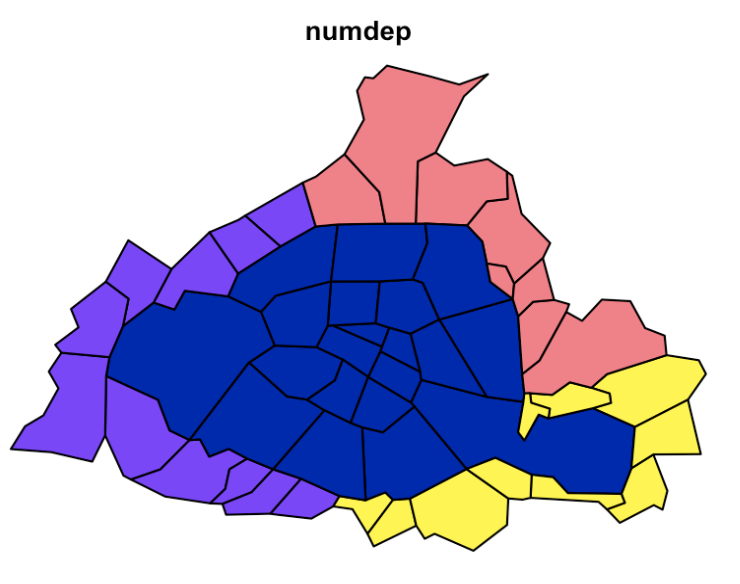
\includegraphics[width=10 cm]{images/Paris_Shape.png}
    \caption{Studied Area color-coded by Department Number}
    \label{fig:Paris_shape}
\end{figure}
 \break
 
 Since Earth is a sphere, a simple application of the Euclidean distance with the points defined by latitude and longitude would not be sufficient. We use the geodetic distance built in the \code{simple features} package to match the format from the Communes d'Île de France shapefile. To do this, first, the borders need to be converted to a line string: if not, the observations inside the Paris department will all be considered to have a distance to the border equal to zero as they are inside of the polygon.
 
 Thus, we can add to the DVF database the "distance to the border" variable for each of the observations. For Diff-in-Disc analysis, the values from this variable are positive in the treatment region and negative in the control region, 

\subsection{Data}
% Pour le mémoire ajouter des explications de comment marche le package sf avec des ss de IDF
For the area of interest and the years 2019, 2020, and 2021 (up until June), we aggregate a total of 283 867 observations before data cleaning. For the analysis, all observations under study must include both longitude and latitude coordinates. That leaves out all observations that are missing one of these values. This amounts to 0.92\% of observations. Additionally, there are instances where a single transaction involving multiple surfaces is registered as multiple entries. To address this, we regroup these "multiple" transactions into a single observation by aggregating the surface values by transaction ID and averaging the distance to the border of the surfaces. This process reduces the size of the database by 18\%. 


We winsorize the top 3\% and bottom 3\% of the observations. Winsorizing is a technique used to deal with outliers in the data by setting, in this case, the values above the 97th percentile and below the 3rd percentile are replaced by the values at these cutoffs. This approach is particularly useful when you want to mitigate the impact of outliers without completely discarding data, as it preserves the overall structure of the dataset while reducing the influence of extreme values. As this study revolves around estimating the Local Average Treatment Effect (LATE), it is crucial to manage extreme values in a way that minimizes their impact on the overall analysis. It is of most pertinence to winsorize in this context because it allows us to reduce the influence of outliers while preserving the integrity of the data. By replacing the extreme values with more moderate ones, we ensure that the analysis remains centered around the average effects, leading to more robust and reliable estimates.

We also replace the missing values (NAs) in the price per squared meter variable using the K-Nearest Neighbors (KNN) method with $k=5$. The KNN algorithm is a non-parametric method where for each missing value, the algorithm identifies the five nearest neighbors in the dataset based on the available features, and the missing value is then imputed based on the average of these neighbors. This method is particularly effective in capturing the local structure of the data, ensuring that the imputed values are consistent with the observed patterns.

Finally, to simplify the data, we only keep the following variables: name of the commune, department code, transaction ID, transaction date, distance to the border, and price per squared meter. This dataset contains 119,297 observations.

Let $D_i$ represent the distance to the border from the property corresponding to the observation $i$. We add the running variable such that : 
\begin{equation}
X_i =
    \begin{cases}
      D_i \text{ if } i\in\text{Paris} \\
      -D_i \text{ else}
    \end{cases}\,.
\end{equation}
\\


However, some observations find themselves outside of France ($12*10^7$ meters away from the border), likely due to inverted latitude and longitude coordinates. To conduct an exhaustive analysis, the sparsity of the data must be reduced. Therefore, all observations further than 100 km away from the border are eliminated. This excludes 2.13\% of observations. Finally, there are 116 753 observations of 7 variables.


\begin{figure}[h!]
    \centering
    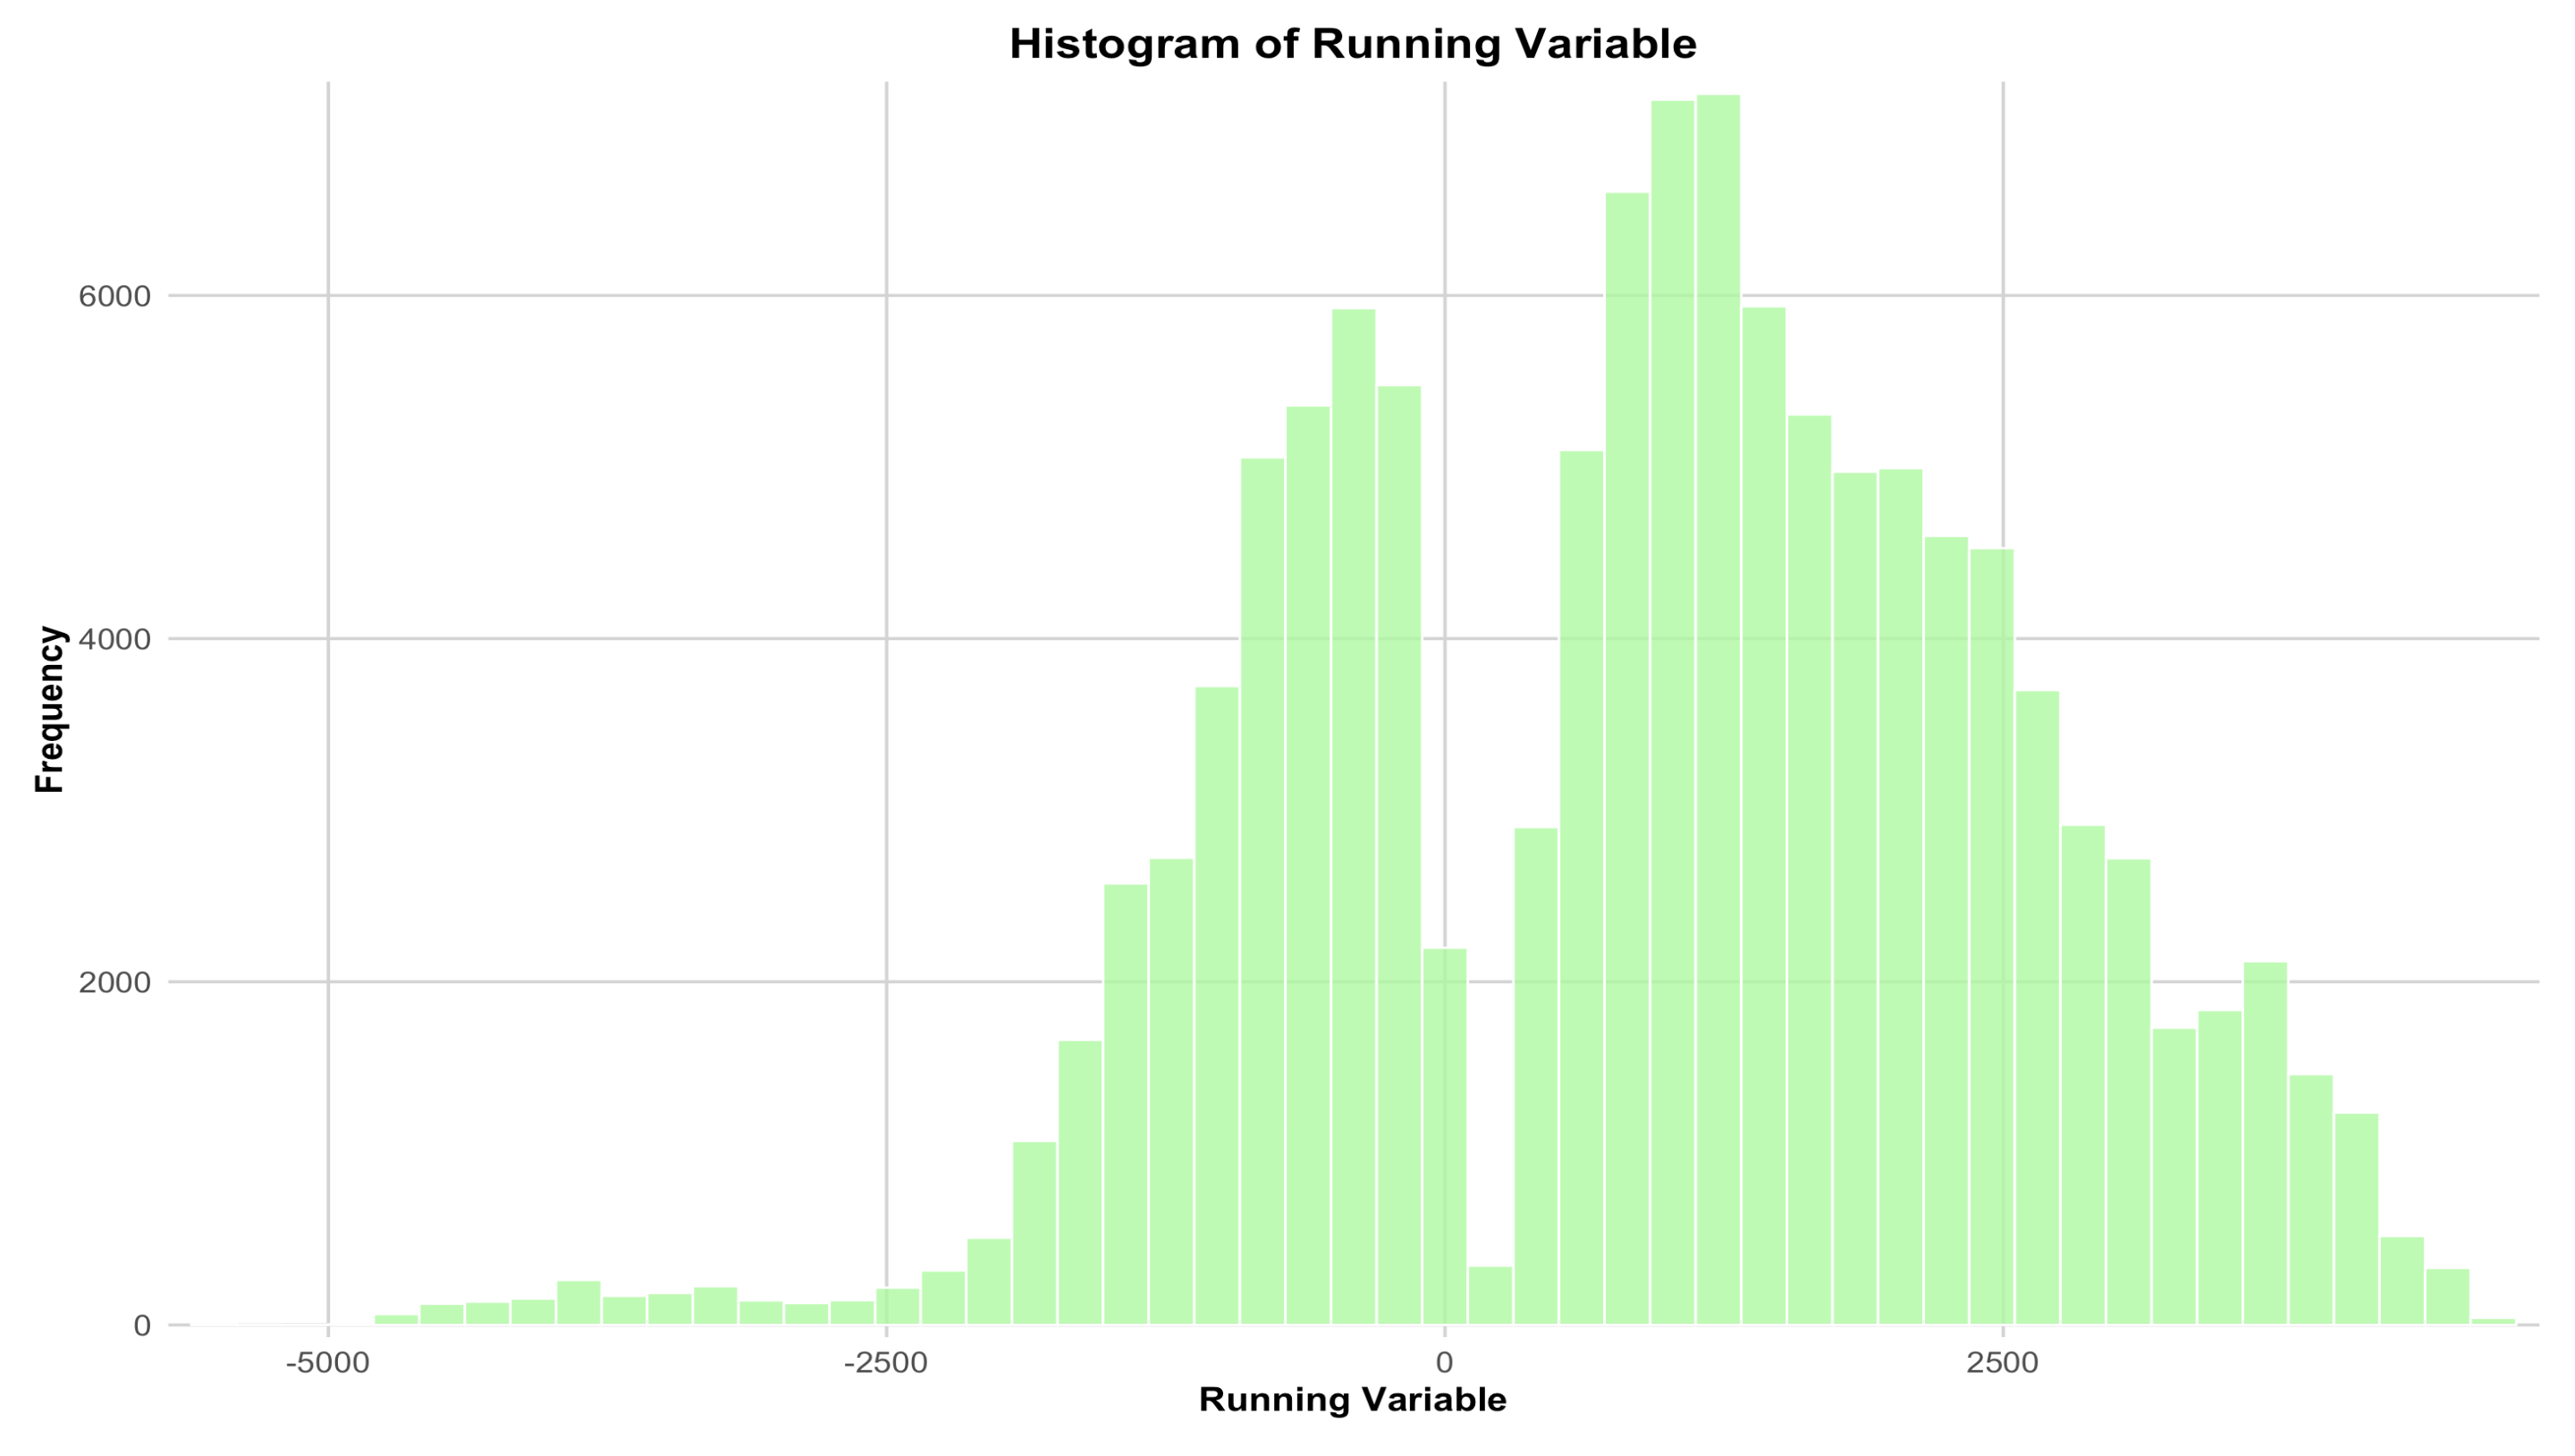
\includegraphics[width=17 cm]{images/RV_hist/RVhist.png}
    \caption{Histogram of the Running Variable within 100km from the border}
    \label{fig:RVhist_post_clean}
\end{figure}
\break


Among these seven variables, I will focus on a more detailed examination of the two key variables used in the Diff-in-Disc analysis: the running variable (the modified distance to the border) and the price per square meter (the outcome variable). I will present general descriptive statistics for these variables, along with a more detailed analysis that explores the characteristics of specific districts and communes. This will include an examination of trends and the overall evolution of these areas, providing deeper insights into the dynamics at play.

\begin{table}[h!]
    \centering
        \begin{tabular}{lr}
            \toprule
            \textbf{Statistic} & \textbf{Value (€/sqm)} \\
            \midrule
            Count      & 116,753.00 \\
            Mean       & 9,271.34 \\
            Median     & 9,433.96 \\
            SD         & 3,495.74 \\
            Min        & 1,429.57 \\
            1st Quartile        & 7,097.56 \\
            3rd Quartile        & 11,425.00 \\
            Max        & 17,051.06 \\
            Skewness   & -0.06 \\
            \bottomrule
            \end{tabular}
    \caption{Descriptive statistics for the Price per Square meter }
    \label{tab:descriptive_stats}
\end{table}

Overall, the descriptive statistics suggest that the price per square meter in the study area is generally high, which is coherent for a very high-demand area like Paris. The slight negative skewness and relatively close mean and median values suggest that while the mean is slightly pulled upwards by extremely high prices, the distribution of prices is fairly symmetric. In addition, there is quite a broad range in prices.
This is further illustrated by the histogram of the variable in Figure \ref{fig:histPPSQM}. The high frequency of extreme prices is a consequence of the winsorization procedure.



\begin{figure}[h!]
    \centering
    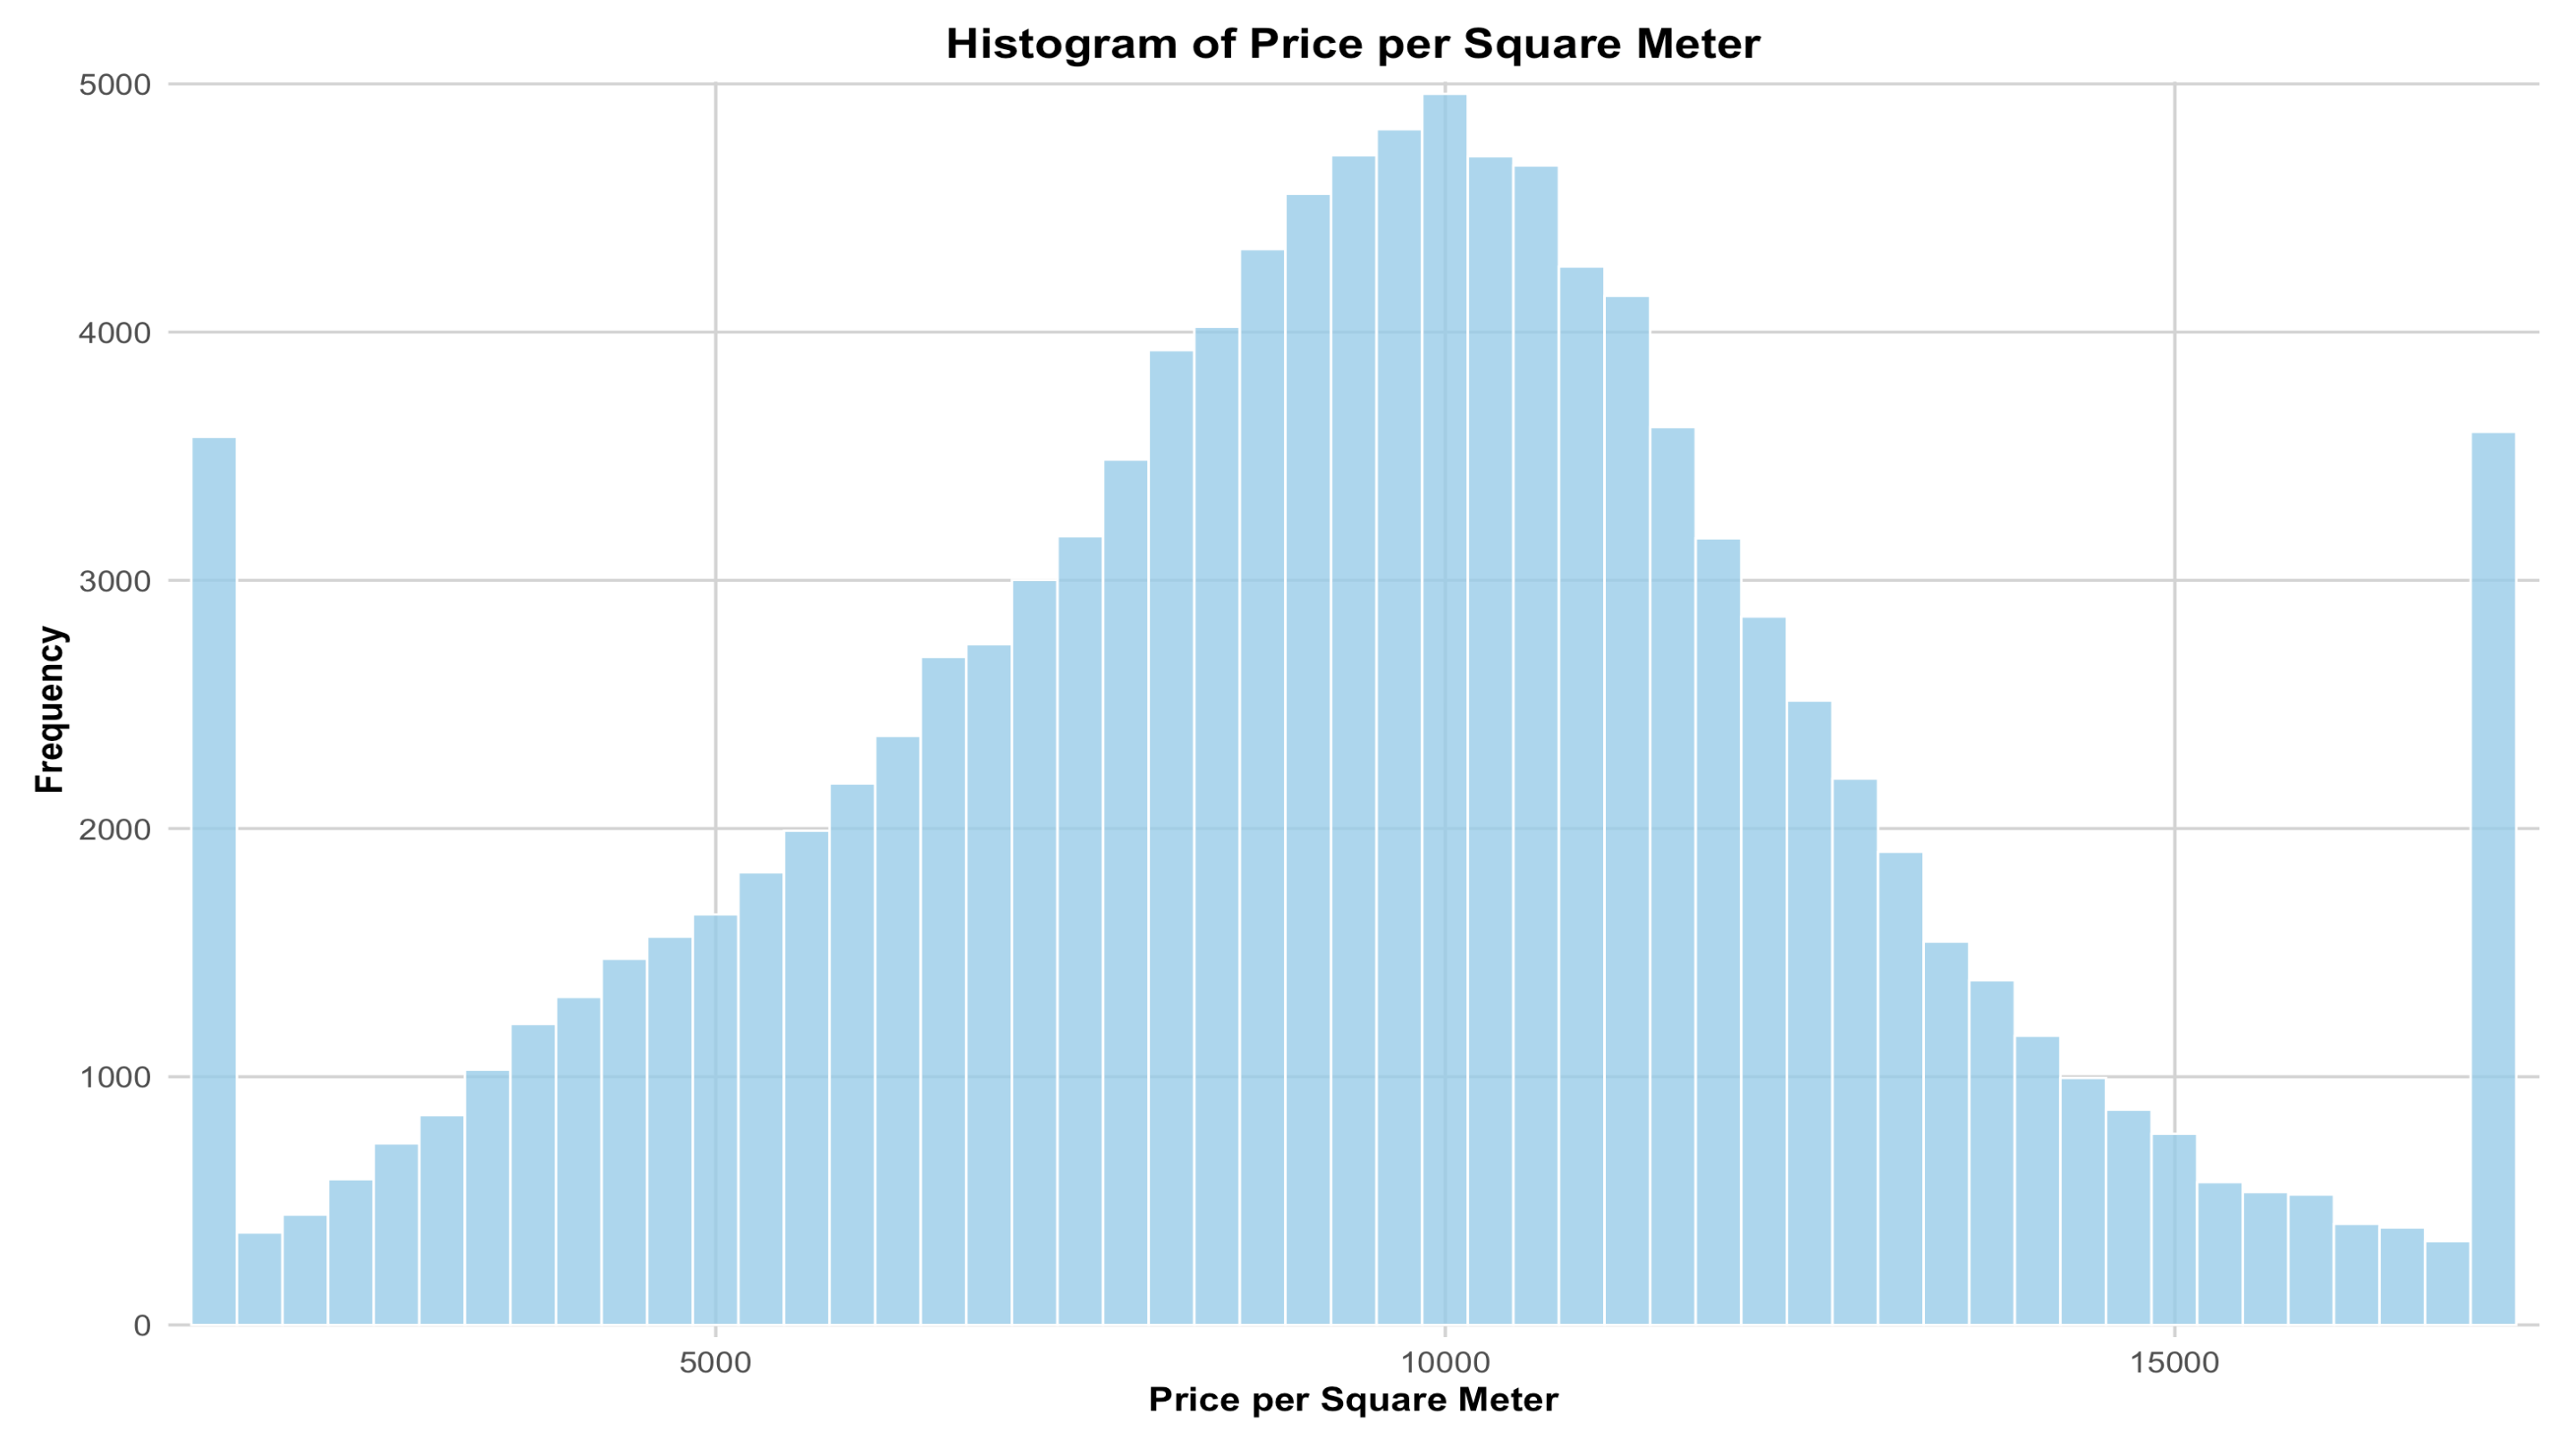
\includegraphics[width=17 cm]{images/RV_hist/PPSQMhist.png}
    \caption{Histogram of the Price per Square Meter in Paris and its surrounding Communes}
    \label{fig:histPPSQM}
\end{figure}
\break

To further illustrate the differences in the square meter price, we can compare the distribution of the square meter in Paris with the distribution of the square meter outside Paris.
\begin{figure}[h!]
    \centering
    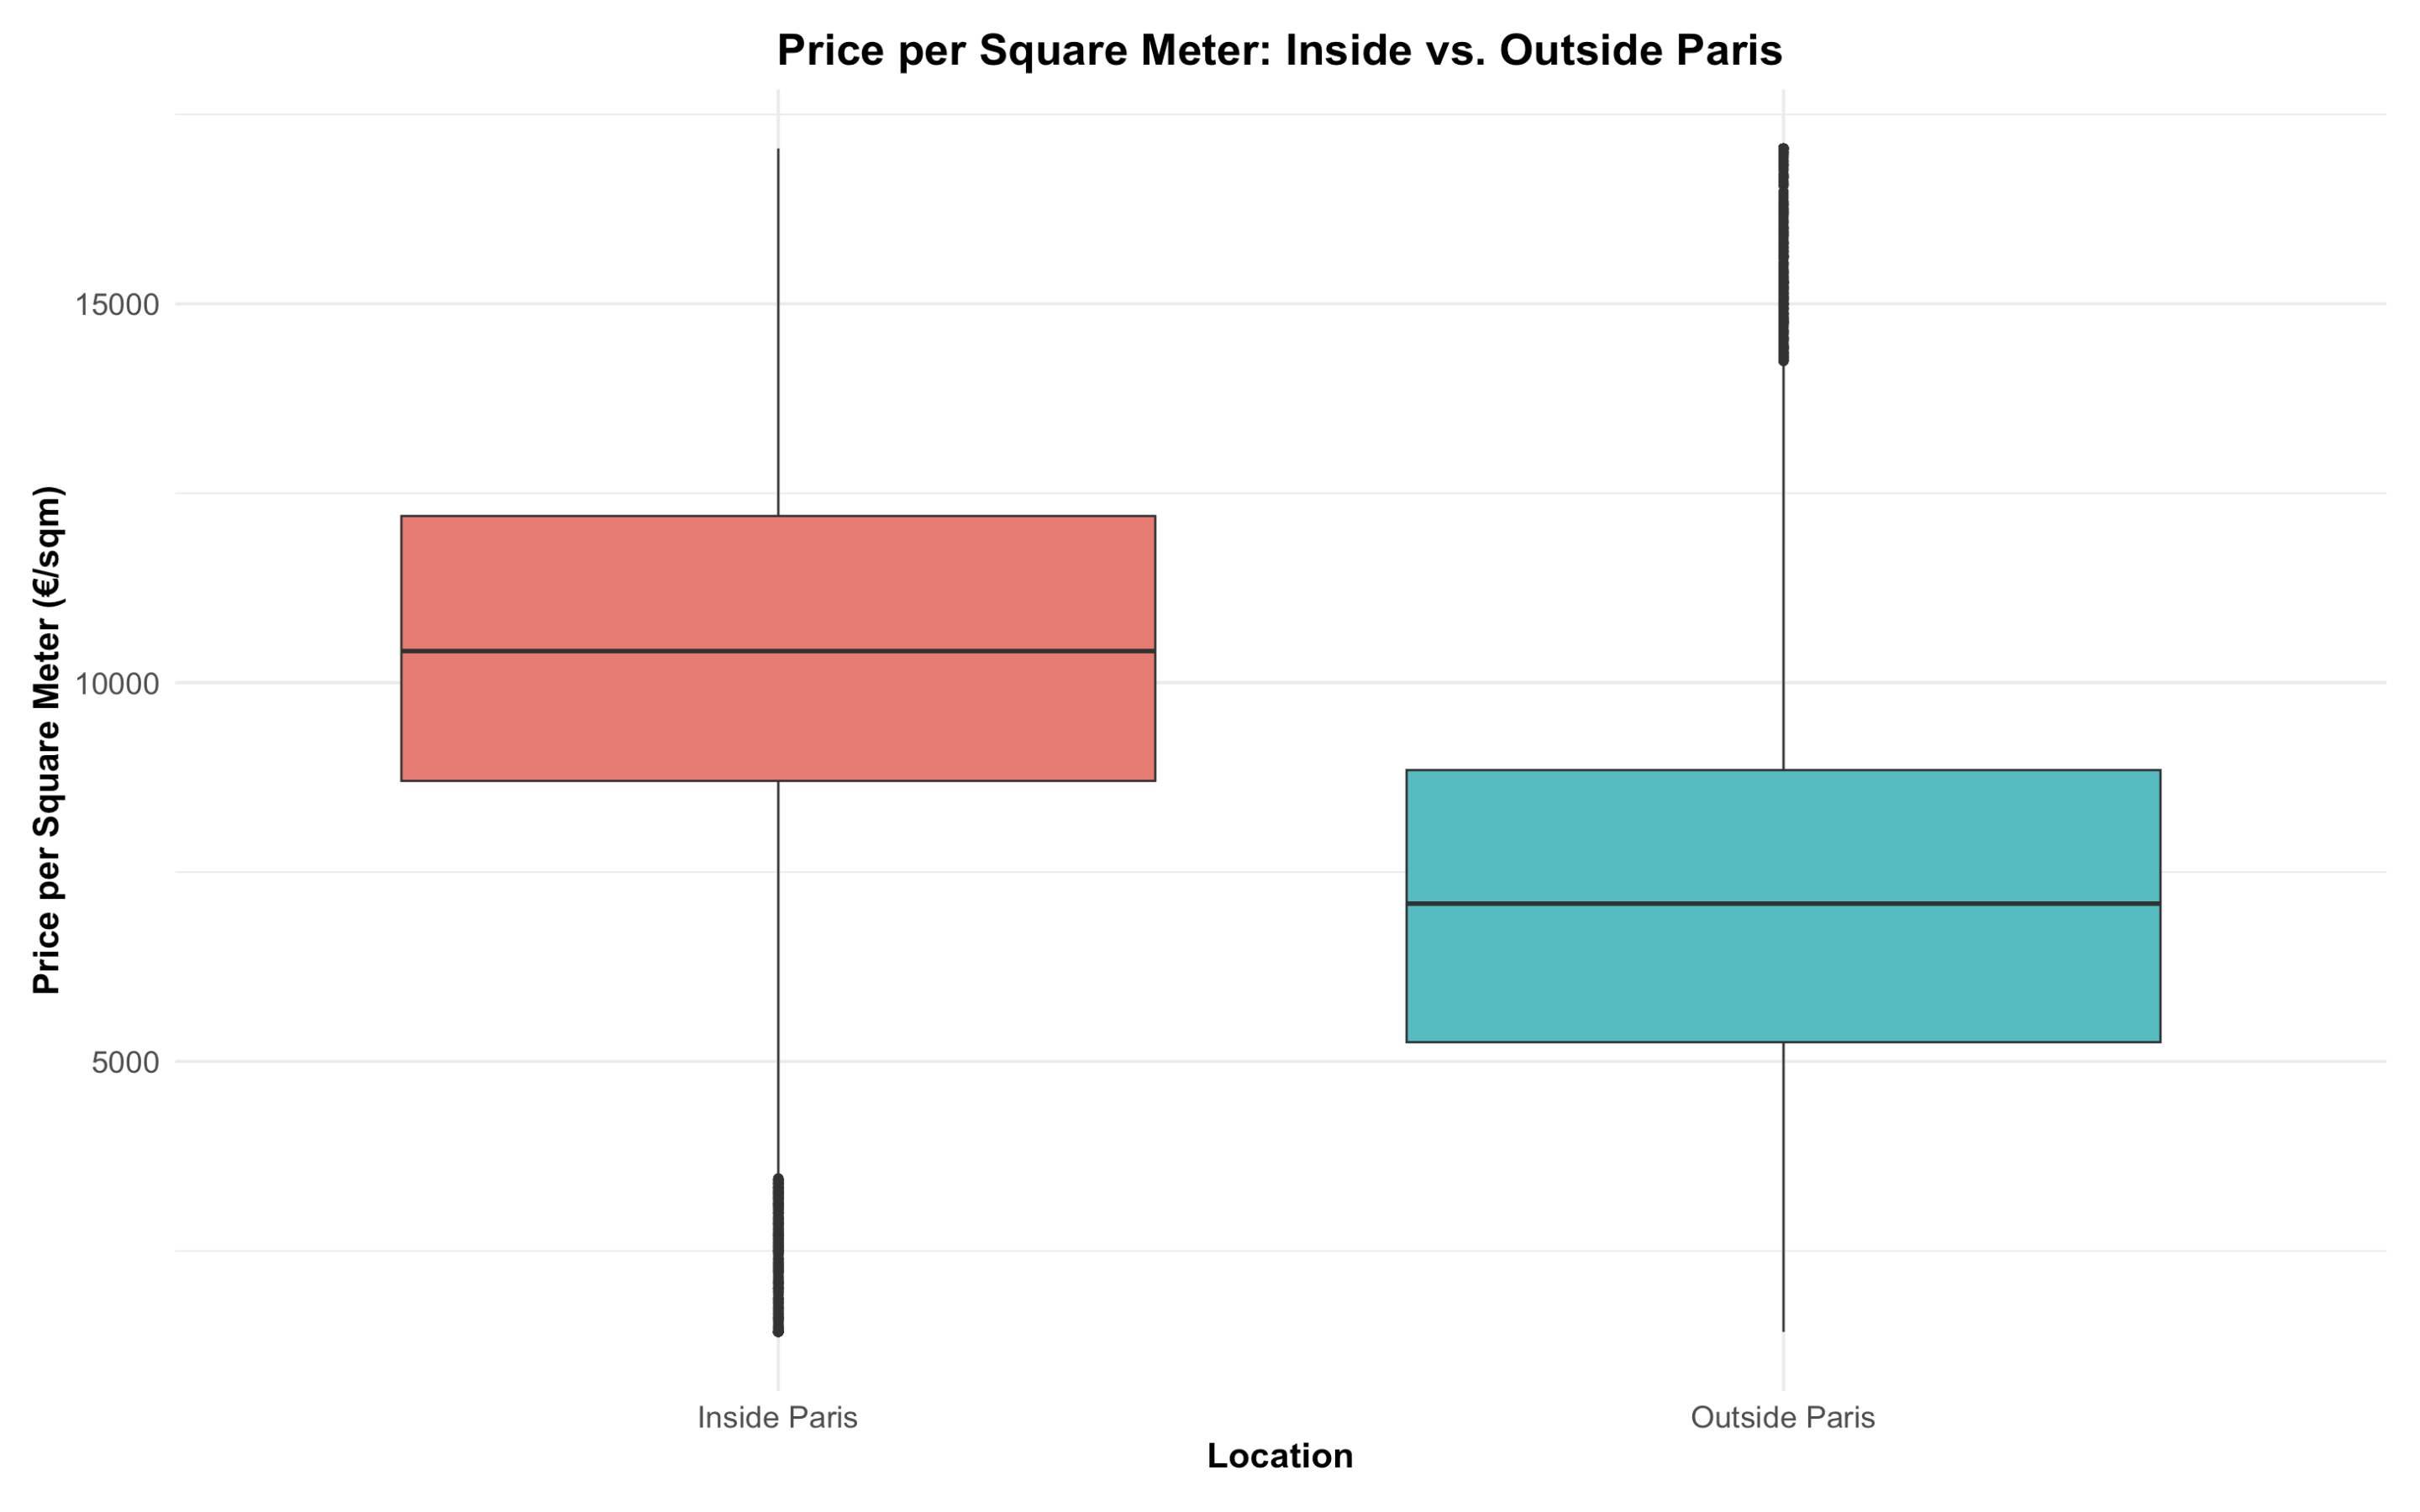
\includegraphics[width=17 cm]{images/Boxplot_inside_outside.png}
    \caption{Comparison between Box Plots Inside and Outside of Paris}
    \label{fig:histPPSQM}
\end{figure}
\break
The two box plots clearly illustrate that the price per square meter is significantly higher in Paris compared to the adjacent communes. The median price per square meter for properties in Paris exceeds €10,000.00, while the median for properties outside Paris is just below €7,500.00. Additionally, the third quartile for properties outside Paris aligns closely with the first quartile for properties within Paris, both around €9,000.00 per square meter. This stark contrast highlights the considerably higher property prices within the city of Paris compared to the surrounding areas. Furthermore, the outliers in Paris are predominantly concentrated at the lower price range, while the outliers outside Paris are mostly found at the higher end of the price spectrum.

To continue with the exploration of the housing market in Paris and its surrounding municipalities, one can take a closer look at the general evolution through the years, illustrated by Figure \ref{fig:evoPPSQM}. 

In 2019, before the implementation of rent control in Paris, the average and median prices per square meter inside Paris were significantly higher than those outside Paris. The median price inside Paris was €10,000, indicating a strong market demand. The lower prices outside Paris, with a median of €6,764.92, reflect the less competitive real estate market in the surrounding communes. There is no immediate effect of the rent control policy in any of the two areas following its implementation in July 2019. In 2020, following the implementation of rent control, the price per square meter inside Paris increased notably, with the mean rising to €10,623.64 and the median to €10,746.21. This increase may suggest that the initial impact of rent control did not depress property prices as might have been anticipated; instead, prices continued to rise, potentially due to the high demand and limited supply within Paris. We cannot gloss over the effects that the COVID-19 pandemic may have had on the evolution of the housing market in both areas. As a matter of fact, in Figure \ref{fig:evoPPSQM} it can be seen that in 2020 there is an inflection point for both locations. 

Outside Paris, the prices also rose, though not as sharply, with the mean and median prices increasing to €7,311.58 and €7,272.73, respectively. This modest increase could be attributed to a spillover effect, where buyers priced out of Paris turned to surrounding communes. The impact of COVID-19 may have also led to a revaluation of suburban areas as more people possibly sought properties outside the city for more space during lockdowns.

By 2021, the price per square meter inside Paris showed a slight decrease in the mean to €10,588.11, but the median remained relatively stable at €10,731.81. This slight decline in the mean could indicate a stabilization of prices following the initial shock of rent control and the ongoing effects of the pandemic. However, the high median suggests that demand for property in Paris remained strong, possibly due to the continued attractiveness of the city.

Outside Paris, the mean and median prices continued to increase to €7,458.70 and €7,485.28, respectively. This rise may reflect the ongoing trend of people moving to suburban areas, a shift accelerated by the pandemic and the potential for more remote work opportunities. It could also illustrate a break in trends between Paris and the outside communes, as Rent Control could have given the adjacent communes a special attractiveness for investors as the price of rent was not controlled.

\begin{figure}[h!]
    \centering
    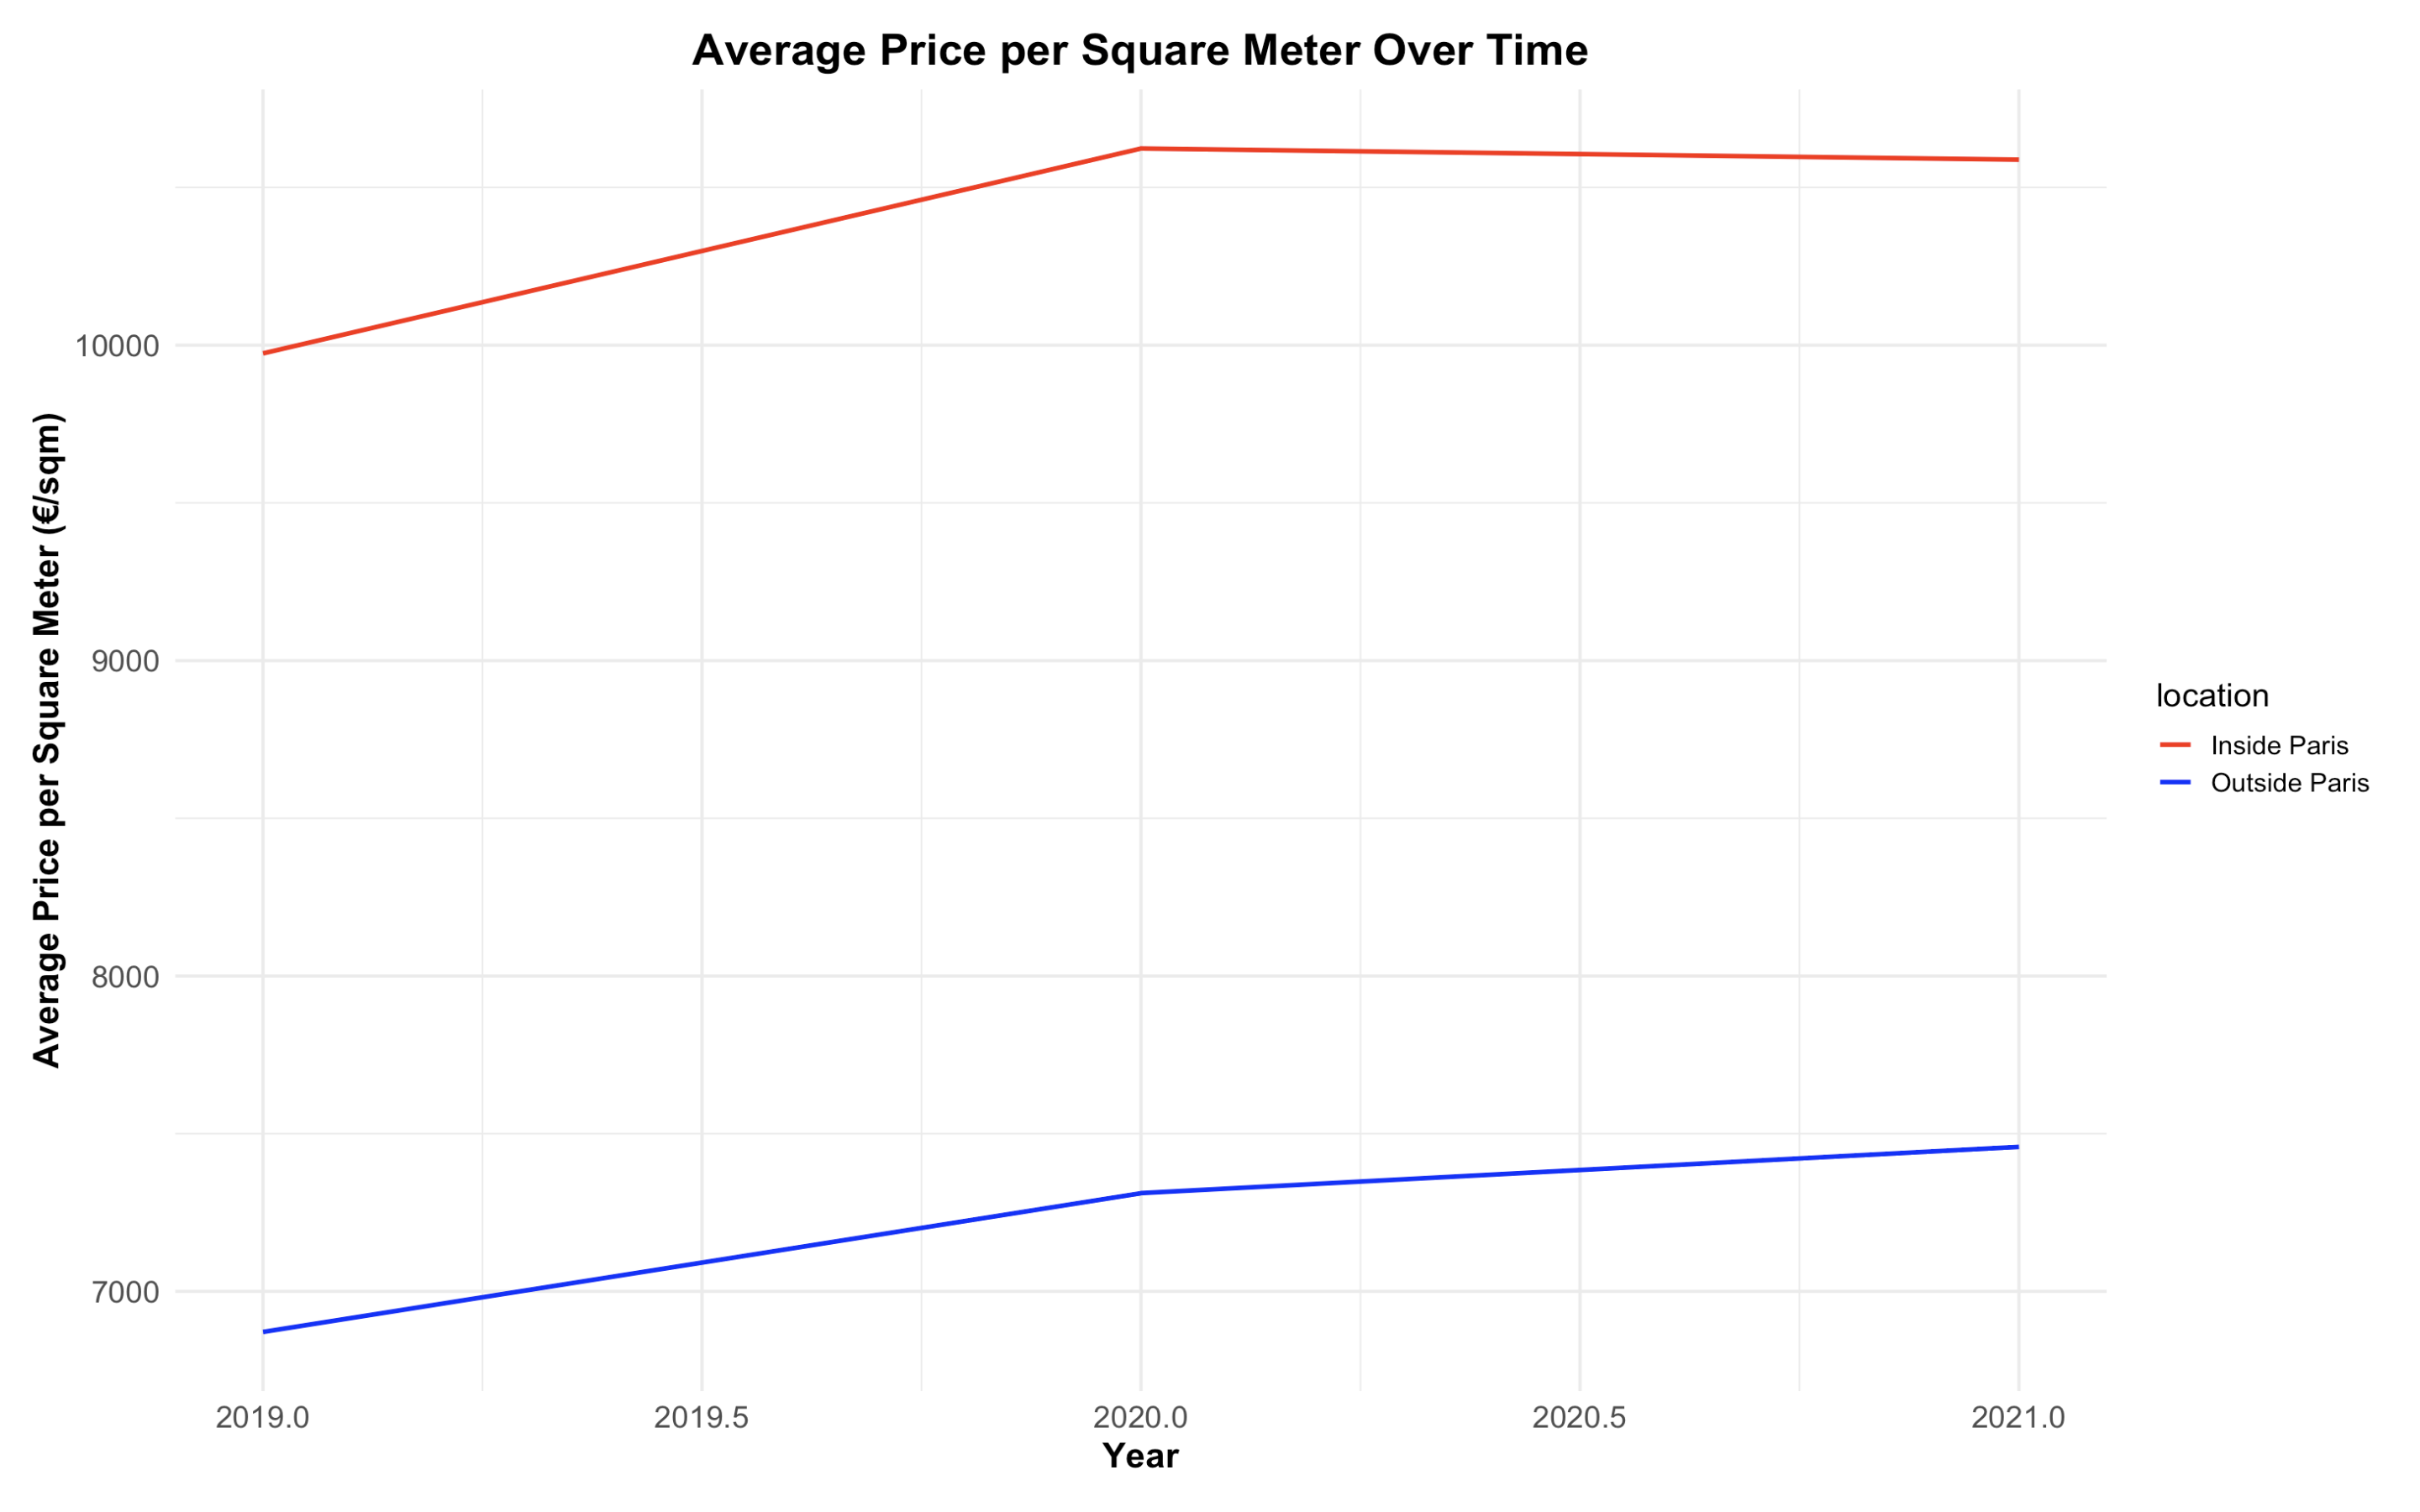
\includegraphics[width=18 cm]{images/PPSQM_evo.png}
    \caption{Average per Square Meter Price Evolution split between Regions}
    \label{fig:evoPPSQM}
\end{figure}
\break

Having explored the trends in average prices per square meter over the years, it is essential to explore how these prices vary across different districts within Paris. While the overall trends provide a broad overview, they do not capture the nuanced differences between specific neighborhoods. 

\begin{table}[!h]
    \centering
    \begin{tabular}{lrrrrr}
        \toprule
        \textbf{District} & \textbf{N} & \textbf{Median (€/sqm)} & \textbf{SD (€/sqm)} & \textbf{Q1 (€/sqm)} & \textbf{Q3 (€/sqm)} \\
        \midrule
        \rowcolor{gray!10}\textbf{Paris 6th} & 1975 & 14339.62 & 4409.57 & 11697.95 & 17051.06 \\
        \textbf{Paris 7th} & 2286 & 14052.29 & 4003.37 & 11766.54 & 16666.67 \\
        \midrule
        \rowcolor{gray!10}\textbf{Paris 4th} & 1302 & 12903.23 & 3975.66 & 10910.99 & 15000.00 \\
        \textbf{Paris 1st} & 782 & 12642.21 & 4067.07 & 10388.46 & 15300.94 \\
        \rowcolor{gray!10}\textbf{Paris 5th} & 2116 & 12349.30 & 3663.61 & 10385.13 & 14167.58 \\
        \textbf{Paris 3rd} & 1749 & 12222.22 & 3956.32 & 10188.68 & 14074.07 \\
        \midrule
        \rowcolor{gray!10}\textbf{Paris 8th} & 1879 & 12037.00 & 4185.29 & 9934.24 & 14044.23 \\
        \textbf{Paris 2nd} & 1314 & 11663.33 & 3790.98 & 9626.73 & 13218.83 \\
        \rowcolor{gray!10}\textbf{Paris 9th} & 3000 & 11344.15 & 3566.98 & 9482.18 & 12973.78 \\
        \textbf{Paris 16th} & 6972 & 11184.29 & 3390.25 & 9600.00 & 12896.46 \\
        \midrule
        \textbf{Paris 17th} & 6888 & 10876.24 & 3148.11 & 9285.71 & 12292.46 \\
        \rowcolor{gray!10}\textbf{Paris 11th} & 6487 & 10555.56 & 2986.46 & 9117.65 & 11838.40 \\
        \textbf{Paris 14th} & 3866 & 10331.92 & 2828.02 & 8995.10 & 11677.14 \\
        \rowcolor{gray!10}\textbf{Paris 15th} & 8016 & 10295.77 & 2696.06 & 8970.59 & 11618.21 \\
        \textbf{Paris 10th} & 4165 & 10284.34 & 3130.35 & 8750.00 & 11617.02 \\
        \midrule
        \rowcolor{gray!10}\textbf{Paris 12th} & 4055 & 9750.00 & 2662.15 & 8453.46 & 10888.89 \\
        \textbf{Paris 18th} & 8551 & 9666.67 & 2940.81 & 8030.66 & 11250.00 \\
        \rowcolor{gray!10}\textbf{Paris 13th} & 3588 & 9451.56 & 2700.52 & 8013.51 & 10724.60 \\
        \midrule
        \textbf{Paris 20th} & 4952 & 9036.04 & 2372.13 & 7867.98 & 10192.31 \\
        \rowcolor{gray!10}\textbf{Paris 19th} & 4327 & 8687.50 & 2515.39 & 7307.69 & 9971.04 \\
        \bottomrule
    \end{tabular}
    \caption{Descriptive Stats for all Paris Districts}
    \label{tab:stat_desc_Arrnd}

\end{table}

Table \ref{tab:stat_desc_Arrnd} offers a closer look at the median prices, variability, and price distribution within various Parisian districts, highlighting the distinct characteristics and market dynamics that influence property values in each area. By analyzing these district-level statistics, we can better understand the spatial variations in the real estate market and how factors such as location, demand, and gentrification contribute to the broader price trends observed in the previous section. We can remark on a certain division that is quite clear between Districts. Generally, these Districts can be regrouped into 6 groups. 

The 6th and 7th Arrondissements stand out as the most expensive areas, with median prices per square meter of €14,339.62 and €14,052.29, respectively. These districts are known for their prime locations, historic architecture, and proximity to cultural landmarks like the Luxembourg Gardens and the Eiffel Tower, which contribute to their high property values. The significant variability in property prices suggests a wide range of property types and conditions within these areas, from luxurious apartments to smaller, perhaps less modernized units, that nonetheless retain amazing property value due to the prestige of the neighborhood.

Paris 1st, 3rd, 4th, and 5th Arrondissements also command high prices, with median values exceeding €12,000 per square meter. The 1st arrondissement, home to the Louvre and Palais Royal, along with the historic Marais area in the 4th arrondissement, reflect their desirability through high property prices. The interquartile ranges in these districts are narrower compared to the top-end districts, indicating more consistent pricing across properties within these central historical areas.

Paris 2nd, 9th, and 16th Arrondissements have median prices slightly above €11,000 per square meter, placing them in the middle tier of Parisian property values. The 16th arrondissement, known for its residential nature and proximity to the Bois de Boulogne, has a somewhat broader distribution of prices, as indicated by its standard deviation. The 8th Arrondissement is an exception in this category, having a median price of €12037.00 and a quite high standard deviation of €4185.29. These districts offer more affordable options compared to the very central or prestigious arrondissements, yet still represent very desirable living areas with good access to amenities and transport.

Paris 10th, 11th, 14th, 15th and 17th Arrondissements have median prices between €10,000 and €11,000 per square meter. These neighborhoods are a blend of residential tranquility and urban convenience.

The Paris 12th, 13th, and 18th arrondissements exhibit median prices below €10,000 per square meter. The relatively higher standard deviations in these areas indicate ongoing shifts in the property market, with significant price variability influenced by the specific neighborhood and proximity to transport hubs. This variability underscores the diverse and contrasted nature of these districts.

Finally, Paris 19th and 20th Arrondissements are the most affordable with median prices of €8,687.50 and €9,036.04 per square meter, respectively. The lower quartiles (Q1) in these districts are also significantly below those of more central areas, indicating that there are still relatively affordable properties available, which could appeal to first-time buyers or those seeking investment opportunities in emerging neighborhoods.

The table illustrates a clear price tendency across Paris, with prices decreasing as one moves away from the central and prestigious western districts towards the eastern and northern districts.
This variability must also be contrasted with the distances of properties from the Paris border in these districts. As shown in Table \ref{tab:dist_minmax}, it is evident that the Parisian districts closest to the border predominantly fall within the lower price tiers.


%leaflet pour cartes interactives si necessaires
%prix médian par arrondissement, prix médian
%motiver : crise de logement, voir l'evaluation de loi pinel ou que sais-je; pourquoi cette loi a ete mise en place, 
%stats desc.
\subsection{Diff-in-Disc Analysis}

Using the same methods as in Section \ref{sec:sim}, this subsection presents the results of the Diff-in-Disc model applied to our dataset, utilizing the three different bandwidth selection methods discussed earlier in this study: the Imbens Plug-in Estimator, the average of two bandwidths, and the Adaptive SGD approach. Each method is applied using both triangular and uniform kernels.

The table below (Table \ref{tab:application_results}) summarizes the estimated bandwidths, treatment effects, and their associated standard deviations for each method and kernel combination. 

The Plug-in Estimator produced relatively wide bandwidths, particularly when using the uniform kernel, resulting in treatment effect estimates that are negative and vary significantly across kernel types. Due to the large variability in the estimates, this conclusion is not statistically robust.

The average of two bandwidths obtained using the \code{rdrobust} package approach also yielded negative treatment effects, although the magnitude of these effects is smaller compared to the Imbens Plug-in Estimator.

Finally, the Adaptive SGD method produced the smallest bandwidths among the three approaches, leading to positive treatment effects. This would be of concern, however, none of these effects are statistically significant. The standard deviations associated with the SGD estimates are larger than those obtained with the other methods, which may suggest increased variability due to the smaller bandwidth size. 

The very large standard deviations associated with each of the estimates of the treatment effects make the effects of the policy statistically insignificant.   


\begin{table}[h]
    \centering
    \caption{Estimated Treatment Effects for Different Optimal Bandwidth and Kernels}
    \begin{tabular}{lcccccc}
        \toprule
        & \multicolumn{2}{c}{Imbens Plug-in Estimator} & \multicolumn{2}{c}{AVG of 2 Bandwidths} & \multicolumn{2}{c}{Adaptive SGD} \\
        \cmidrule(lr){2-3} \cmidrule(lr){4-5} \cmidrule(lr){6-7}
        \multirow{2}{*} & Triangular & Uniform & Triangular & Uniform & Triangular & Uniform \\
        \midrule
        Bandwidth & 444.43 & 698.15 & 673.56 & 637.13 & 230.96 & 231.69 \\ 
        Treatment Effect & -510.29 & -88.74 & -356.45 & -134.16 & 291.46 & 274.57 \\
        & \scriptsize{(569.31)} & \scriptsize{(339.28)} & \scriptsize{(361.20)} & \scriptsize{(390.76)} & \scriptsize{(953.5)} & \scriptsize{(1117.23)} \\
        \bottomrule
    \end{tabular}
    \label{tab:application_results}
\end{table}

The analysis of the Diff-in-Disc model applied to the impact of the rent control policy on property prices in Paris does not provide statistically significant evidence of a clear effect, whether positive or negative. The large standard deviations associated with the treatment effect estimates suggest that the observed variations could be due to random noise rather than a systematic impact of the policy. This could be due to perturbations caused by the COVID-19 pandemic and all of its underlying effects.
Given these limitations, the study cannot conclusively determine the impact of the rent control policy on property prices within the time frame analyzed.

\newpage
\section{Conclusion}
This paper has explored the application of the Difference-in-Discontinuities (Diff-in-Disc) methodology in evaluating the impact of rent control policies on property prices within Paris. By employing various bandwidth selection methods and kernels, we aimed to rigorously estimate the local average treatment effect. However, the results were marked by substantial variability and large standard deviations, leading to statistically insignificant conclusions about the impact of the policy. 

Our analysis revealed that the Diff-in-Disc approach, while powerful, is highly sensitive to the choice of bandwidth and kernel, which significantly influences the estimated treatment effects. The study also highlighted the inherent challenges in dealing with real-world data, such as the impact of external factors like the COVID-19 pandemic, which may obscure the true effects of policy interventions.

Despite the lack of statistically significant findings, this study provides valuable insights into the dynamics of property prices in Paris. It underscores the need for robust statistical tools when evaluating policy impacts. The complexity of the application and the lack of robustness in the standard deviations could be solved by a clustering algorithm (i.e. max\_p\_tabu algorithm from the \href{https://geodacenter.github.io/rgeoda/reference/maxp_tabu.html}{\code{rgeoda} package}). 

Furthermore, the application results may evidence that the Adaptive SGD algorithm might need reinforcement to try finding bandwidths leading to more robust estimates. The choice of the AdaGrad learning rate for the proposed Adaptive SGD may be subject to criticism, as other learning rates could potentially be better suited to addressing the challenges of a non-convex optimization problem.

While the current study has focused on a standard Diff-in-Disc model, several extensions could enhance and expand the applicability of the Diff-in-Disc methodology: properly formalizing the fuzzy design into the Diff-in-Disc framework could account for situations where treatment assignment is not strictly binary or where there is partial compliance with the treatment conditions. This extension would allow for more realistic modeling of scenarios and further case applications where policy implementation is uneven or subject to exceptions. Another valuable extension would incorporate a time-variant running variable ($X_{it}$) into the model. This approach would be particularly useful in contexts where the running variable is not static over time, allowing the analysis to capture the dynamic nature of policy impacts as the relevant conditions evolve.

Finally, to further strengthen the Diff-in-Disc methodology, particularly concerning the derivative equivalence assumption, it is essential to incorporate validity tests. Such tests could involve testing for Derivative Equivalence by implementing specific tests to verify the assumption that the derivatives of the regression functions on either side of the cutoff are indeed equivalent. This would help ensure that the Diff-in-Disc methodology is indeed suited for a particular application.
Withal, conducting robustness checks by varying the bandwidth and examining the consistency of the treatment effects across different model specifications could provide further confidence in the validity of the results or highlight areas where the model might need refinement.
% Ajouter une explication du max_tabu pour les clusters

\newpage
\section{Bibliography}
\printbibliography % Print the bibliography

\newpage
\section{Appendix}

\begin{table}[h!]
    \centering
    \begin{tabular}{lrr}
        \toprule
        \textbf{Statistic} & \textbf{Inside Paris} & \textbf{Outside Paris} \\
        \midrule
        N          & 78,270.00 & 38,483.00 \\
        Mean       & 1,848.02  & 910.26 \\
        Median     & 1,679.17  & 726.30 \\
        SD         & 985.27    & 794.05 \\
        Min        & 17.01     & 0.03 \\
        Max        & 4,634.66  & 5,571.90 \\
        \bottomrule
    \end{tabular}
    \caption{Descriptive statistics for distance to the border from properties inside and outside Paris}
    \label{tab:RV_stats}
\end{table}


\begin{table}[!h]
    \centering
    \caption{Descriptive Stats for the Surrounding Municipalities}
    \begin{tabular}{lrrrrr}
        \toprule
        \textbf{Commune} & \textbf{N} & \textbf{Median Price (€/sqm)} & \textbf{SD (€/sqm)} & \textbf{Q1 (€/sqm)} & \textbf{Q3 (€/sqm)} \\
        \midrule
        \rowcolor{gray!10}\textbf{Neuilly-sur-Seine} & 2355 & 10932.203 & 3100.368 & 9423.077 & 12381.385 \\
        \textbf{Levallois-Perret} & 2586 & 9559.412 & 2393.359 & 8255.814 & 10543.565 \\
        \rowcolor{gray!10}\textbf{Vincennes} & 2100 & 8850.287 & 2555.405 & 7500.000 & 10000.000 \\
        \textbf{Saint-Mandé} & 859 & 8833.333 & 2474.274 & 7715.168 & 9911.999 \\
        \rowcolor{gray!10}\textbf{Boulogne-Billancourt} & 4745 & 8813.559 & 2385.924 & 7702.703 & 9915.730 \\
        \textbf{Issy-les-Moulineaux} & 1910 & 7993.985 & 2102.226 & 6734.783 & 8947.368 \\
        \rowcolor{gray!10}\textbf{Charenton-le-Pont} & 944 & 7816.506 & 1985.889 & 6646.163 & 8775.829 \\
        \midrule
        \textbf{Montrouge} & 1585 & 7457.576 & 2063.043 & 6275.862 & 8523.810 \\
        \rowcolor{gray!10}\textbf{Puteaux} & 1511 & 7227.541 & 1963.772 & 6132.765 & 8139.212 \\
        \textbf{Suresnes} & 1356 & 6962.500 & 1929.609 & 5988.542 & 7773.386 \\
        \rowcolor{gray!10}\textbf{Clichy} & 1719 & 6945.055 & 2258.630 & 5658.805 & 7960.355 \\
        \textbf{Malakoff} & 580 & 6756.757 & 2156.190 & 5793.139 & 7590.818 \\
        \rowcolor{gray!10}\textbf{Les Lilas} & 597 & 6750.000 & 1871.711 & 5750.000 & 7685.185 \\
        \textbf{Vanves} & 828 & 6718.041 & 1740.051 & 5927.198 & 7594.444 \\
        \midrule
        \rowcolor{gray!10}\textbf{Saint-Cloud} & 912 & 6713.173 & 1848.740 & 5932.333 & 7641.257 \\
        \textbf{Le Pré-Saint-Gervais} & 440 & 6295.648 & 1871.659 & 5284.962 & 7072.723 \\
        \rowcolor{gray!10}\textbf{Nogent-sur-Marne} & 1383 & 6171.875 & 1812.327 & 5300.000 & 7007.463 \\
        \textbf{Montreuil} & 2460 & 6166.667 & 2273.278 & 4601.105 & 7371.709 \\
        \rowcolor{gray!10}\textbf{Saint-Maurice} & 485 & 6052.632 & 1946.624 & 5097.368 & 7162.162 \\
        \textbf{Pantin} & 1399 & 5896.552 & 1936.979 & 4642.857 & 6914.237 \\
        \rowcolor{gray!10}\textbf{Le Kremlin-Bicêtre} & 529 & 5813.953 & 1537.136 & 4992.647 & 6500.000 \\
        \midrule
        \textbf{Gentilly} & 280 & 5732.117 & 1726.265 & 5087.981 & 6668.605 \\
        \rowcolor{gray!10}\textbf{Fontenay-sous-Bois} & 1147 & 5703.125 & 1890.832 & 4429.476 & 6756.156 \\
        \textbf{Joinville-le-Pont} & 527 & 5441.176 & 1490.860 & 4721.117 & 6204.167 \\
        \rowcolor{gray!10}\textbf{Bagnolet} & 675 & 5205.128 & 1692.679 & 4073.425 & 6244.595 \\
        \textbf{Ivry-sur-Seine} & 1150 & 4949.194 & 1548.688 & 4167.339 & 5760.046 \\
        \rowcolor{gray!10}\textbf{Saint-Denis} & 2006 & 3893.256 & 1561.640 & 3123.859 & 4576.143 \\
        \textbf{Aubervilliers} & 1415 & 3666.667 & 1747.538 & 2934.188 & 4446.429 \\
        \bottomrule
    \end{tabular}
\end{table}
\label{tab:dist_minmax}
\break

\newpage
\begin{longtable}{lrr}
\caption{Minimal and Maximal Distances to the Border for all Paris Districts and Surrounding Communes} \\
\toprule
\textbf{Commune} & \textbf{Minimal Distance to Border (m)} & \textbf{Maximum Distance to Border (m)} \\
\midrule
\endfirsthead

\multicolumn{3}{c}{{\tablename\ \thetable{} -- continued from previous page}} \\
\toprule
\textbf{Commune} & \textbf{Minimal Distance to Border (m)} & \textbf{Maximum Distance to Border (m)} \\
\midrule
\endhead

\midrule \multicolumn{3}{r}{{Continued on next page}} \\
\endfoot

\bottomrule
\endlastfoot

Montrouge               & 0.03   & 1396.30 \\
Neuilly-sur-Seine       & 0.41   & 1719.00 \\
Boulogne-Billancourt    & 0.54   & 1962.57 \\
Vincennes               & 1.05   & 1078.78 \\
Nogent-sur-Marne        & 1.11   & 2130.72 \\
Saint-Mandé             & 1.16   & 395.46  \\
Issy-les-Moulineaux     & 1.42   & 2109.33 \\
Gentilly                & 1.60   & 776.38  \\
Charenton-le-Pont       & 2.24   & 829.92  \\
Le Pré-Saint-Gervais    & 3.83   & 718.02  \\
Levallois-Perret        & 4.40   & 1425.84 \\
Saint-Maurice           & 5.88   & 663.87  \\
\midrule
Paris 19e Arrondissement & 17.01  & 2231.43 \\
Paris 17e Arrondissement & 18.08  & 1855.90 \\
Les Lilas               & 23.41  & 1376.09 \\
Bagnolet                & 27.08  & 1743.86 \\
Aubervilliers           & 32.49  & 2460.26 \\
Clichy                  & 37.50  & 1452.08 \\
Ivry-sur-Seine          & 38.38  & 2429.91 \\
Pantin                  & 39.58  & 2302.35 \\
Le Kremlin-Bicêtre      & 39.71  & 1462.40 \\
Montreuil               & 39.77  & 3795.72 \\
Paris 16e Arrondissement & 52.15  & 2617.89 \\
Puteaux                 & 54.18  & 1694.80 \\
Vanves                  & 54.61  & 1638.37 \\
Fontenay-sous-Bois      & 62.73  & 2941.21 \\
Joinville-le-Pont       & 66.01  & 1480.13 \\
Malakoff                & 69.17  & 1989.19 \\
\midrule
Paris 18e Arrondissement & 107.38 & 2106.60 \\
Saint-Cloud             & 156.42 & 2192.68 \\
Suresnes                & 195.63 & 1880.51 \\
Saint-Denis             & 207.59 & 5571.90 \\
Paris 15e Arrondissement & 212.14 & 2799.46 \\
Paris 20e Arrondissement & 253.83 & 2202.07 \\
Paris 13e Arrondissement & 269.41 & 2362.12 \\
Paris 14e Arrondissement & 316.06 & 2445.04 \\
Paris 12e Arrondissement & 330.01 & 3234.89 \\
\midrule
Paris 8e Arrondissement  & 1262.14 & 3224.12 \\
Paris 11e Arrondissement & 1280.57 & 3442.16 \\
Paris 9e Arrondissement  & 1900.83 & 3370.93 \\
Paris 10e Arrondissement & 1939.47 & 3585.29 \\
Paris 5e Arrondissement  & 2110.46 & 3936.72 \\
\midrule
Paris 7e Arrondissement  & 2325.49 & 4243.56 \\
Paris 6e Arrondissement  & 2469.24 & 4223.29 \\
Paris 4e Arrondissement  & 3020.15 & 4603.54 \\
Paris 1er Arrondissement & 3236.31 & 4634.66 \\
Paris 3e Arrondissement  & 3285.26 & 4359.36 \\
Paris 2e Arrondissement  & 3306.91 & 4211.60 \\
\end{longtable}

\end{document}

% LACUNES : blocage - cercher a fond tout seul; question d'organisation
